\documentclass{whiteboard}
\begin{document}
\begin{frame}[plain,t]
\bbcover{Timus 1280}{Topological Sorting}{Prof. Edson Alves}{Faculdade UnB Gama}

\end{frame}
\begin{frame}[plain,t]
\vspace*{\fill}

\bbenglish{Michael wants to win the world championship in programming and decided to study $N$ subjects (for convenience we will number these subjects from $1$ to $N$). Michael has worked out a study plan for this purpose. But it turned out that certain subjects may be studied only after others. So, Michael’s coach analyzed all subjects and prepared a list of $M$ limitations in the form ``$s_i\ u_i$'' $(1\leq s_i, u_i\leq N;$ $i = 1, 2, \ldots, M)$, which means that subject $s_i$ must be studied before subject $u_i$.}

\vspace{0.1in}

\bbenglish{Your task is to verify if the order of subjects being studied is correct.}

\vspace*{\fill}
\end{frame}
\begin{frame}[plain,t]
\vspace*{\fill}

\bbtext{Michael quer vencer o campeonato mundial de programação e decidiu estudar $N$ assuntos (de forma conveniente, nós iremos numerar estes assuntos de $1$ a $N$). Michael trabalhou em um plano de estudos para este objetivo. Mas acontece que certos assuntos só devem ser estudados após alguns outros. Assim, o técnico de Michael analisou os assuntos e preparou uma lista de $M$ limitações na forma ``$s_i\ u_i$'' $(1\leq s_i, u_i\leq N;$ $i = 1, 2, \ldots, M)$, o que significa que o assunto $s_i$ deve ser estudado antes do assunto $u_i$.}

\vspace{0.1in}

\bbtext{Sua tarefa é verificar se a ordem dos assuntos a serem estudados está correta.}

\vspace*{\fill}
\end{frame}
\begin{frame}[plain,t]
\vspace*{\fill}

\bbbold{Remark.} \bbenglish{It may appear that it’s impossible to find the correct order of subjects within the given limitations. In this case any subject order worked out by Michael is incorrect.}

\vspace{0.2in}

\bbbold{Limitations}

\vspace{0.1in}

$1\leq N\leq 1000; 0\leq M\leq 100000.$

\vspace*{\fill}
\end{frame}
\begin{frame}[plain,t]
\vspace*{\fill}

\bbbold{Observação.} \bbtext{Pode ser impossível encontrar uma ordem correta para os assuntos que atenda as limitações dadas. Neste caso qualquer ordem de assuntos produzida por Michael estará incorreta.}

\vspace{0.2in}

\bbbold{Limitações}

\vspace{0.1in}

$1\leq N\leq 1000; 0\leq M\leq 100000.$

\vspace*{\fill}
\end{frame}
\begin{frame}[plain,t]
\vspace*{\fill}

\bbbold{Input}

\vspace{0.1in}

\bbenglish{The first line contains two integers $N$ and $M$ ($N$ is the number of the subjects, $M$ is the number of the limitations). The next $M$ lines contain pairs $s_i, u_i$, which describe the order of subjects: subject $s_i$ must be studied before $u_i$. Further there is a sequence of $N$ unique numbers ranging from $1$ to $N$ -- the proposed study plan.}

\vspace{0.2in}

\bbbold{Output}

\vspace{0.1in}

\bbenglish{Output a single word ``\texttt{YES}'' or ``\texttt{NO}''. ``\texttt{YES}'' means that the proposed order is correct and has no contradictions with the given limitations. ``\texttt{NO}'' means that the order is incorrect.}

\vspace*{\fill}
\end{frame}
\begin{frame}[plain,t]
\vspace*{\fill}

\bbbold{Entrada}

\vspace{0.1in}

\bbtext{A primeira linha contém dois inteiros $N$ e $M$ ($N$ é o número de assuntos, $M$ é o número de limitações). As próximas $M$ linhas contém pares $s_i, u_i$, os quais descrevem a ordem dos assuntos: o assunto $s_i$ deve ser estudado antes do assunto $u_i$. A seguir há uma sequência de $N$ inteiros únicos no intervalo de $1$ a $N$ -- o plano de estudo proposto.}

\vspace{0.2in}

\bbbold{Saída}

\vspace{0.1in}

\bbtext{Imprima uma única palavra: ``\texttt{YES}'' ou ``\texttt{NO}''. ``\texttt{YES}'' significa que a ordem proposta está correta e que não há contradições com as limitações dadas. ``\texttt{NO}'' significa que a ordem está incorreta.}

\vspace*{\fill}
\end{frame}
\begin{frame}[plain,t]
\begin{tikzpicture}
\node[draw,opacity=0] at (0, 0) {x};
\node[draw,opacity=0] at (14, 8) {x};

	\node[anchor=west] (header) at (0, 7.0) { \bbbold{Exemplo de entrada e saída} };

\end{tikzpicture}
\end{frame}
\begin{frame}[plain,t]
\begin{tikzpicture}
\node[draw,opacity=0] at (0, 0) {x};
\node[draw,opacity=0] at (14, 8) {x};

	\node[anchor=west] (header) at (0, 7.0) { \bbbold{Exemplo de entrada e saída} };


	\node[anchor=west] (line1) at (1.0, 6.0) { \bbtext{\texttt{5 6} } };

\end{tikzpicture}
\end{frame}
\begin{frame}[plain,t]
\begin{tikzpicture}
\node[draw,opacity=0] at (0, 0) {x};
\node[draw,opacity=0] at (14, 8) {x};

	\node[anchor=west] (header) at (0, 7.0) { \bbbold{Exemplo de entrada e saída} };


	\node[anchor=west] (line1) at (1.0, 6.0) { \bbtext{\texttt{5 6} } };


	\draw[->,color=BBViolet] (1.25, 5.0) to  (1.25, 5.75);

	\node[] (r) at (1.25, 4.75) { \footnotesize \bbcomment{\# de assuntos} };

\end{tikzpicture}
\end{frame}
\begin{frame}[plain,t]
\begin{tikzpicture}
\node[draw,opacity=0] at (0, 0) {x};
\node[draw,opacity=0] at (14, 8) {x};

	\node[anchor=west] (header) at (0, 7.0) { \bbbold{Exemplo de entrada e saída} };


	\node[anchor=west] (line1) at (1.0, 6.0) { \bbtext{\texttt{5 6} } };


	\draw[->,color=BBViolet] (1.65, 5.0) to  (1.65, 5.75);

	\node[] (r) at (1.65, 4.75) { \footnotesize \bbcomment{\# de limitações} };



\end{tikzpicture}
\end{frame}
\begin{frame}[plain,t]
\begin{tikzpicture}
\node[draw,opacity=0] at (0, 0) {x};
\node[draw,opacity=0] at (14, 8) {x};

	\node[anchor=west] (header) at (0, 7.0) { \bbbold{Exemplo de entrada e saída} };


	\node[anchor=west] (line1) at (1.0, 6.0) { \bbtext{\texttt{5 6} } };







	\node[draw,very thick,circle] (node1) at (7.0, 4.0) { \bbtext{1} };

	\node[draw,very thick,circle] (node2) at (10.0, 7.0) { \bbtext{2} };

	\node[draw,very thick,circle] (node3) at (13.0, 4.0) { \bbtext{3} };

	\node[draw,very thick,circle] (node4) at (12.0, 1.0) { \bbtext{4} };

	\node[draw,very thick,circle] (node5) at (8.0, 1.0) { \bbtext{5} };
\end{tikzpicture}
\end{frame}
\begin{frame}[plain,t]
\begin{tikzpicture}
\node[draw,opacity=0] at (0, 0) {x};
\node[draw,opacity=0] at (14, 8) {x};

	\node[anchor=west] (header) at (0, 7.0) { \bbbold{Exemplo de entrada e saída} };


	\node[anchor=west] (line1) at (1.0, 6.0) { \bbtext{\texttt{5 6} } };







	\node[draw,very thick,circle] (node1) at (7.0, 4.0) { \bbtext{1} };

	\node[draw,very thick,circle] (node2) at (10.0, 7.0) { \bbtext{2} };

	\node[draw,very thick,circle] (node3) at (13.0, 4.0) { \bbtext{3} };

	\node[draw,very thick,circle] (node4) at (12.0, 1.0) { \bbtext{4} };

	\node[draw,very thick,circle] (node5) at (8.0, 1.0) { \bbtext{5} };

	\node[anchor=west] (line2) at (1.0, 5.5) { \bbtext{\texttt{1 3} } };

\end{tikzpicture}
\end{frame}
\begin{frame}[plain,t]
\begin{tikzpicture}
\node[draw,opacity=0] at (0, 0) {x};
\node[draw,opacity=0] at (14, 8) {x};

	\node[anchor=west] (header) at (0, 7.0) { \bbbold{Exemplo de entrada e saída} };


	\node[anchor=west] (line1) at (1.0, 6.0) { \bbtext{\texttt{5 6} } };


	\draw[->,color=BBViolet] (1.25, 4.25) to  (1.25, 5.25);

	\node[] (r) at (1.25, 4.0) { \footnotesize \bbcomment{$s_i$} };




	\node[draw,very thick,circle] (node1) at (7.0, 4.0) { \bbtext{1} };

	\node[draw,very thick,circle] (node2) at (10.0, 7.0) { \bbtext{2} };

	\node[draw,very thick,circle] (node3) at (13.0, 4.0) { \bbtext{3} };

	\node[draw,very thick,circle] (node4) at (12.0, 1.0) { \bbtext{4} };

	\node[draw,very thick,circle] (node5) at (8.0, 1.0) { \bbtext{5} };

	\node[anchor=west] (line2) at (1.0, 5.5) { \bbtext{\texttt{1 3} } };



\end{tikzpicture}
\end{frame}
\begin{frame}[plain,t]
\begin{tikzpicture}
\node[draw,opacity=0] at (0, 0) {x};
\node[draw,opacity=0] at (14, 8) {x};

	\node[anchor=west] (header) at (0, 7.0) { \bbbold{Exemplo de entrada e saída} };


	\node[anchor=west] (line1) at (1.0, 6.0) { \bbtext{\texttt{5 6} } };


	\draw[->,color=BBViolet] (1.65, 4.25) to  (1.65, 5.25);

	\node[] (r) at (1.65, 4.0) { \footnotesize \bbcomment{$u_i$} };




	\node[draw,very thick,circle] (node1) at (7.0, 4.0) { \bbtext{1} };

	\node[draw,very thick,circle] (node2) at (10.0, 7.0) { \bbtext{2} };

	\node[draw,very thick,circle] (node3) at (13.0, 4.0) { \bbtext{3} };

	\node[draw,very thick,circle] (node4) at (12.0, 1.0) { \bbtext{4} };

	\node[draw,very thick,circle] (node5) at (8.0, 1.0) { \bbtext{5} };

	\node[anchor=west] (line2) at (1.0, 5.5) { \bbtext{\texttt{1 3} } };





\end{tikzpicture}
\end{frame}
\begin{frame}[plain,t]
\begin{tikzpicture}
\node[draw,opacity=0] at (0, 0) {x};
\node[draw,opacity=0] at (14, 8) {x};

	\node[anchor=west] (header) at (0, 7.0) { \bbbold{Exemplo de entrada e saída} };


	\node[anchor=west] (line1) at (1.0, 6.0) { \bbtext{\texttt{5 6} } };







	\node[draw,very thick,circle] (node1) at (7.0, 4.0) { \bbtext{1} };

	\node[draw,very thick,circle] (node2) at (10.0, 7.0) { \bbtext{2} };

	\node[draw,very thick,circle] (node3) at (13.0, 4.0) { \bbtext{3} };

	\node[draw,very thick,circle] (node4) at (12.0, 1.0) { \bbtext{4} };

	\node[draw,very thick,circle] (node5) at (8.0, 1.0) { \bbtext{5} };

	\node[anchor=west] (line2) at (1.0, 5.5) { \bbtext{\texttt{1 3} } };






	\draw[thick,-latex](node1) to (node3);

\end{tikzpicture}
\end{frame}
\begin{frame}[plain,t]
\begin{tikzpicture}
\node[draw,opacity=0] at (0, 0) {x};
\node[draw,opacity=0] at (14, 8) {x};

	\node[anchor=west] (header) at (0, 7.0) { \bbbold{Exemplo de entrada e saída} };


	\node[anchor=west] (line1) at (1.0, 6.0) { \bbtext{\texttt{5 6} } };







	\node[draw,very thick,circle] (node1) at (7.0, 4.0) { \bbtext{1} };

	\node[draw,very thick,circle] (node2) at (10.0, 7.0) { \bbtext{2} };

	\node[draw,very thick,circle] (node3) at (13.0, 4.0) { \bbtext{3} };

	\node[draw,very thick,circle] (node4) at (12.0, 1.0) { \bbtext{4} };

	\node[draw,very thick,circle] (node5) at (8.0, 1.0) { \bbtext{5} };

	\node[anchor=west] (line2) at (1.0, 5.5) { \bbtext{\texttt{1 3} } };






	\draw[thick,-latex](node1) to (node3);


	\node[anchor=west] (line3) at (1.0, 5.0) { \bbtext{\texttt{1 4} } };

\end{tikzpicture}
\end{frame}
\begin{frame}[plain,t]
\begin{tikzpicture}
\node[draw,opacity=0] at (0, 0) {x};
\node[draw,opacity=0] at (14, 8) {x};

	\node[anchor=west] (header) at (0, 7.0) { \bbbold{Exemplo de entrada e saída} };


	\node[anchor=west] (line1) at (1.0, 6.0) { \bbtext{\texttt{5 6} } };







	\node[draw,very thick,circle] (node1) at (7.0, 4.0) { \bbtext{1} };

	\node[draw,very thick,circle] (node2) at (10.0, 7.0) { \bbtext{2} };

	\node[draw,very thick,circle] (node3) at (13.0, 4.0) { \bbtext{3} };

	\node[draw,very thick,circle] (node4) at (12.0, 1.0) { \bbtext{4} };

	\node[draw,very thick,circle] (node5) at (8.0, 1.0) { \bbtext{5} };

	\node[anchor=west] (line2) at (1.0, 5.5) { \bbtext{\texttt{1 3} } };






	\draw[thick,-latex](node1) to (node3);


	\node[anchor=west] (line3) at (1.0, 5.0) { \bbtext{\texttt{1 4} } };


	\draw[thick,-latex](node1) to (node4);

\end{tikzpicture}
\end{frame}
\begin{frame}[plain,t]
\begin{tikzpicture}
\node[draw,opacity=0] at (0, 0) {x};
\node[draw,opacity=0] at (14, 8) {x};

	\node[anchor=west] (header) at (0, 7.0) { \bbbold{Exemplo de entrada e saída} };


	\node[anchor=west] (line1) at (1.0, 6.0) { \bbtext{\texttt{5 6} } };







	\node[draw,very thick,circle] (node1) at (7.0, 4.0) { \bbtext{1} };

	\node[draw,very thick,circle] (node2) at (10.0, 7.0) { \bbtext{2} };

	\node[draw,very thick,circle] (node3) at (13.0, 4.0) { \bbtext{3} };

	\node[draw,very thick,circle] (node4) at (12.0, 1.0) { \bbtext{4} };

	\node[draw,very thick,circle] (node5) at (8.0, 1.0) { \bbtext{5} };

	\node[anchor=west] (line2) at (1.0, 5.5) { \bbtext{\texttt{1 3} } };






	\draw[thick,-latex](node1) to (node3);


	\node[anchor=west] (line3) at (1.0, 5.0) { \bbtext{\texttt{1 4} } };


	\draw[thick,-latex](node1) to (node4);


	\node[anchor=west] (line4) at (1.0, 4.5) { \bbtext{\texttt{3 5} } };

\end{tikzpicture}
\end{frame}
\begin{frame}[plain,t]
\begin{tikzpicture}
\node[draw,opacity=0] at (0, 0) {x};
\node[draw,opacity=0] at (14, 8) {x};

	\node[anchor=west] (header) at (0, 7.0) { \bbbold{Exemplo de entrada e saída} };


	\node[anchor=west] (line1) at (1.0, 6.0) { \bbtext{\texttt{5 6} } };







	\node[draw,very thick,circle] (node1) at (7.0, 4.0) { \bbtext{1} };

	\node[draw,very thick,circle] (node2) at (10.0, 7.0) { \bbtext{2} };

	\node[draw,very thick,circle] (node3) at (13.0, 4.0) { \bbtext{3} };

	\node[draw,very thick,circle] (node4) at (12.0, 1.0) { \bbtext{4} };

	\node[draw,very thick,circle] (node5) at (8.0, 1.0) { \bbtext{5} };

	\node[anchor=west] (line2) at (1.0, 5.5) { \bbtext{\texttt{1 3} } };






	\draw[thick,-latex](node1) to (node3);


	\node[anchor=west] (line3) at (1.0, 5.0) { \bbtext{\texttt{1 4} } };


	\draw[thick,-latex](node1) to (node4);


	\node[anchor=west] (line4) at (1.0, 4.5) { \bbtext{\texttt{3 5} } };


	\draw[thick,-latex](node3) to (node5);
\end{tikzpicture}
\end{frame}
\begin{frame}[plain,t]
\begin{tikzpicture}
\node[draw,opacity=0] at (0, 0) {x};
\node[draw,opacity=0] at (14, 8) {x};

	\node[anchor=west] (header) at (0, 7.0) { \bbbold{Exemplo de entrada e saída} };


	\node[anchor=west] (line1) at (1.0, 6.0) { \bbtext{\texttt{5 6} } };







	\node[draw,very thick,circle] (node1) at (7.0, 4.0) { \bbtext{1} };

	\node[draw,very thick,circle] (node2) at (10.0, 7.0) { \bbtext{2} };

	\node[draw,very thick,circle] (node3) at (13.0, 4.0) { \bbtext{3} };

	\node[draw,very thick,circle] (node4) at (12.0, 1.0) { \bbtext{4} };

	\node[draw,very thick,circle] (node5) at (8.0, 1.0) { \bbtext{5} };

	\node[anchor=west] (line2) at (1.0, 5.5) { \bbtext{\texttt{1 3} } };






	\draw[thick,-latex](node1) to (node3);


	\node[anchor=west] (line3) at (1.0, 5.0) { \bbtext{\texttt{1 4} } };


	\draw[thick,-latex](node1) to (node4);


	\node[anchor=west] (line4) at (1.0, 4.5) { \bbtext{\texttt{3 5} } };


	\draw[thick,-latex](node3) to (node5);

	\node[anchor=west] (line5) at (1.0, 4.0) { \bbtext{\texttt{5 2} } };

\end{tikzpicture}
\end{frame}
\begin{frame}[plain,t]
\begin{tikzpicture}
\node[draw,opacity=0] at (0, 0) {x};
\node[draw,opacity=0] at (14, 8) {x};

	\node[anchor=west] (header) at (0, 7.0) { \bbbold{Exemplo de entrada e saída} };


	\node[anchor=west] (line1) at (1.0, 6.0) { \bbtext{\texttt{5 6} } };







	\node[draw,very thick,circle] (node1) at (7.0, 4.0) { \bbtext{1} };

	\node[draw,very thick,circle] (node2) at (10.0, 7.0) { \bbtext{2} };

	\node[draw,very thick,circle] (node3) at (13.0, 4.0) { \bbtext{3} };

	\node[draw,very thick,circle] (node4) at (12.0, 1.0) { \bbtext{4} };

	\node[draw,very thick,circle] (node5) at (8.0, 1.0) { \bbtext{5} };

	\node[anchor=west] (line2) at (1.0, 5.5) { \bbtext{\texttt{1 3} } };






	\draw[thick,-latex](node1) to (node3);


	\node[anchor=west] (line3) at (1.0, 5.0) { \bbtext{\texttt{1 4} } };


	\draw[thick,-latex](node1) to (node4);


	\node[anchor=west] (line4) at (1.0, 4.5) { \bbtext{\texttt{3 5} } };


	\draw[thick,-latex](node3) to (node5);

	\node[anchor=west] (line5) at (1.0, 4.0) { \bbtext{\texttt{5 2} } };


	\draw[thick,-latex](node5) to (node2);

\end{tikzpicture}
\end{frame}
\begin{frame}[plain,t]
\begin{tikzpicture}
\node[draw,opacity=0] at (0, 0) {x};
\node[draw,opacity=0] at (14, 8) {x};

	\node[anchor=west] (header) at (0, 7.0) { \bbbold{Exemplo de entrada e saída} };


	\node[anchor=west] (line1) at (1.0, 6.0) { \bbtext{\texttt{5 6} } };







	\node[draw,very thick,circle] (node1) at (7.0, 4.0) { \bbtext{1} };

	\node[draw,very thick,circle] (node2) at (10.0, 7.0) { \bbtext{2} };

	\node[draw,very thick,circle] (node3) at (13.0, 4.0) { \bbtext{3} };

	\node[draw,very thick,circle] (node4) at (12.0, 1.0) { \bbtext{4} };

	\node[draw,very thick,circle] (node5) at (8.0, 1.0) { \bbtext{5} };

	\node[anchor=west] (line2) at (1.0, 5.5) { \bbtext{\texttt{1 3} } };






	\draw[thick,-latex](node1) to (node3);


	\node[anchor=west] (line3) at (1.0, 5.0) { \bbtext{\texttt{1 4} } };


	\draw[thick,-latex](node1) to (node4);


	\node[anchor=west] (line4) at (1.0, 4.5) { \bbtext{\texttt{3 5} } };


	\draw[thick,-latex](node3) to (node5);

	\node[anchor=west] (line5) at (1.0, 4.0) { \bbtext{\texttt{5 2} } };


	\draw[thick,-latex](node5) to (node2);


	\node[anchor=west] (line6) at (1.0, 3.5) { \bbtext{\texttt{4 2} } };

\end{tikzpicture}
\end{frame}
\begin{frame}[plain,t]
\begin{tikzpicture}
\node[draw,opacity=0] at (0, 0) {x};
\node[draw,opacity=0] at (14, 8) {x};

	\node[anchor=west] (header) at (0, 7.0) { \bbbold{Exemplo de entrada e saída} };


	\node[anchor=west] (line1) at (1.0, 6.0) { \bbtext{\texttt{5 6} } };







	\node[draw,very thick,circle] (node1) at (7.0, 4.0) { \bbtext{1} };

	\node[draw,very thick,circle] (node2) at (10.0, 7.0) { \bbtext{2} };

	\node[draw,very thick,circle] (node3) at (13.0, 4.0) { \bbtext{3} };

	\node[draw,very thick,circle] (node4) at (12.0, 1.0) { \bbtext{4} };

	\node[draw,very thick,circle] (node5) at (8.0, 1.0) { \bbtext{5} };

	\node[anchor=west] (line2) at (1.0, 5.5) { \bbtext{\texttt{1 3} } };






	\draw[thick,-latex](node1) to (node3);


	\node[anchor=west] (line3) at (1.0, 5.0) { \bbtext{\texttt{1 4} } };


	\draw[thick,-latex](node1) to (node4);


	\node[anchor=west] (line4) at (1.0, 4.5) { \bbtext{\texttt{3 5} } };


	\draw[thick,-latex](node3) to (node5);

	\node[anchor=west] (line5) at (1.0, 4.0) { \bbtext{\texttt{5 2} } };


	\draw[thick,-latex](node5) to (node2);


	\node[anchor=west] (line6) at (1.0, 3.5) { \bbtext{\texttt{4 2} } };


	\draw[thick,-latex](node4) to (node2);

\end{tikzpicture}
\end{frame}
\begin{frame}[plain,t]
\begin{tikzpicture}
\node[draw,opacity=0] at (0, 0) {x};
\node[draw,opacity=0] at (14, 8) {x};

	\node[anchor=west] (header) at (0, 7.0) { \bbbold{Exemplo de entrada e saída} };


	\node[anchor=west] (line1) at (1.0, 6.0) { \bbtext{\texttt{5 6} } };







	\node[draw,very thick,circle] (node1) at (7.0, 4.0) { \bbtext{1} };

	\node[draw,very thick,circle] (node2) at (10.0, 7.0) { \bbtext{2} };

	\node[draw,very thick,circle] (node3) at (13.0, 4.0) { \bbtext{3} };

	\node[draw,very thick,circle] (node4) at (12.0, 1.0) { \bbtext{4} };

	\node[draw,very thick,circle] (node5) at (8.0, 1.0) { \bbtext{5} };

	\node[anchor=west] (line2) at (1.0, 5.5) { \bbtext{\texttt{1 3} } };






	\draw[thick,-latex](node1) to (node3);


	\node[anchor=west] (line3) at (1.0, 5.0) { \bbtext{\texttt{1 4} } };


	\draw[thick,-latex](node1) to (node4);


	\node[anchor=west] (line4) at (1.0, 4.5) { \bbtext{\texttt{3 5} } };


	\draw[thick,-latex](node3) to (node5);

	\node[anchor=west] (line5) at (1.0, 4.0) { \bbtext{\texttt{5 2} } };


	\draw[thick,-latex](node5) to (node2);


	\node[anchor=west] (line6) at (1.0, 3.5) { \bbtext{\texttt{4 2} } };


	\draw[thick,-latex](node4) to (node2);


	\node[anchor=west] (line7) at (1.0, 3.0) { \bbtext{\texttt{1 2} } };

\end{tikzpicture}
\end{frame}
\begin{frame}[plain,t]
\begin{tikzpicture}
\node[draw,opacity=0] at (0, 0) {x};
\node[draw,opacity=0] at (14, 8) {x};

	\node[anchor=west] (header) at (0, 7.0) { \bbbold{Exemplo de entrada e saída} };


	\node[anchor=west] (line1) at (1.0, 6.0) { \bbtext{\texttt{5 6} } };







	\node[draw,very thick,circle] (node1) at (7.0, 4.0) { \bbtext{1} };

	\node[draw,very thick,circle] (node2) at (10.0, 7.0) { \bbtext{2} };

	\node[draw,very thick,circle] (node3) at (13.0, 4.0) { \bbtext{3} };

	\node[draw,very thick,circle] (node4) at (12.0, 1.0) { \bbtext{4} };

	\node[draw,very thick,circle] (node5) at (8.0, 1.0) { \bbtext{5} };

	\node[anchor=west] (line2) at (1.0, 5.5) { \bbtext{\texttt{1 3} } };






	\draw[thick,-latex](node1) to (node3);


	\node[anchor=west] (line3) at (1.0, 5.0) { \bbtext{\texttt{1 4} } };


	\draw[thick,-latex](node1) to (node4);


	\node[anchor=west] (line4) at (1.0, 4.5) { \bbtext{\texttt{3 5} } };


	\draw[thick,-latex](node3) to (node5);

	\node[anchor=west] (line5) at (1.0, 4.0) { \bbtext{\texttt{5 2} } };


	\draw[thick,-latex](node5) to (node2);


	\node[anchor=west] (line6) at (1.0, 3.5) { \bbtext{\texttt{4 2} } };


	\draw[thick,-latex](node4) to (node2);


	\node[anchor=west] (line7) at (1.0, 3.0) { \bbtext{\texttt{1 2} } };


	\draw[thick,-latex](node1) to (node2);

\end{tikzpicture}
\end{frame}
\begin{frame}[plain,t]
\begin{tikzpicture}
\node[draw,opacity=0] at (0, 0) {x};
\node[draw,opacity=0] at (14, 8) {x};

	\node[anchor=west] (header) at (0, 7.0) { \bbbold{Exemplo de entrada e saída} };


	\node[anchor=west] (line1) at (1.0, 6.0) { \bbtext{\texttt{5 6} } };







	\node[draw,very thick,circle] (node1) at (7.0, 4.0) { \bbtext{1} };

	\node[draw,very thick,circle] (node2) at (10.0, 7.0) { \bbtext{2} };

	\node[draw,very thick,circle] (node3) at (13.0, 4.0) { \bbtext{3} };

	\node[draw,very thick,circle] (node4) at (12.0, 1.0) { \bbtext{4} };

	\node[draw,very thick,circle] (node5) at (8.0, 1.0) { \bbtext{5} };

	\node[anchor=west] (line2) at (1.0, 5.5) { \bbtext{\texttt{1 3} } };






	\draw[thick,-latex](node1) to (node3);


	\node[anchor=west] (line3) at (1.0, 5.0) { \bbtext{\texttt{1 4} } };


	\draw[thick,-latex](node1) to (node4);


	\node[anchor=west] (line4) at (1.0, 4.5) { \bbtext{\texttt{3 5} } };


	\draw[thick,-latex](node3) to (node5);

	\node[anchor=west] (line5) at (1.0, 4.0) { \bbtext{\texttt{5 2} } };


	\draw[thick,-latex](node5) to (node2);


	\node[anchor=west] (line6) at (1.0, 3.5) { \bbtext{\texttt{4 2} } };


	\draw[thick,-latex](node4) to (node2);


	\node[anchor=west] (line7) at (1.0, 3.0) { \bbtext{\texttt{1 2} } };


	\draw[thick,-latex](node1) to (node2);


	\node[anchor=west] (line8) at (1.0, 2.5) { \bbtext{\texttt{1 3 4 5 2} } };

\end{tikzpicture}
\end{frame}
\begin{frame}[plain,t]
\begin{tikzpicture}
\node[draw,opacity=0] at (0, 0) {x};
\node[draw,opacity=0] at (14, 8) {x};

	\node[anchor=west] (header) at (0, 7.0) { \bbbold{Exemplo de entrada e saída} };


	\node[anchor=west] (line1) at (1.0, 6.0) { \bbtext{\texttt{5 6} } };


	\draw[->,color=BBViolet] (2.05, 1.25) to  (2.05, 2.25);

	\node[] (r) at (2.05, 1.0) { \footnotesize \bbcomment{ordem proposta} };




	\node[draw,very thick,circle] (node1) at (7.0, 4.0) { \bbtext{1} };

	\node[draw,very thick,circle] (node2) at (10.0, 7.0) { \bbtext{2} };

	\node[draw,very thick,circle] (node3) at (13.0, 4.0) { \bbtext{3} };

	\node[draw,very thick,circle] (node4) at (12.0, 1.0) { \bbtext{4} };

	\node[draw,very thick,circle] (node5) at (8.0, 1.0) { \bbtext{5} };

	\node[anchor=west] (line2) at (1.0, 5.5) { \bbtext{\texttt{1 3} } };






	\draw[thick,-latex](node1) to (node3);


	\node[anchor=west] (line3) at (1.0, 5.0) { \bbtext{\texttt{1 4} } };


	\draw[thick,-latex](node1) to (node4);


	\node[anchor=west] (line4) at (1.0, 4.5) { \bbtext{\texttt{3 5} } };


	\draw[thick,-latex](node3) to (node5);

	\node[anchor=west] (line5) at (1.0, 4.0) { \bbtext{\texttt{5 2} } };


	\draw[thick,-latex](node5) to (node2);


	\node[anchor=west] (line6) at (1.0, 3.5) { \bbtext{\texttt{4 2} } };


	\draw[thick,-latex](node4) to (node2);


	\node[anchor=west] (line7) at (1.0, 3.0) { \bbtext{\texttt{1 2} } };


	\draw[thick,-latex](node1) to (node2);


	\node[anchor=west] (line8) at (1.0, 2.5) { \bbtext{\texttt{1 3 4 5 2} } };



\end{tikzpicture}
\end{frame}
\begin{frame}[plain,t]
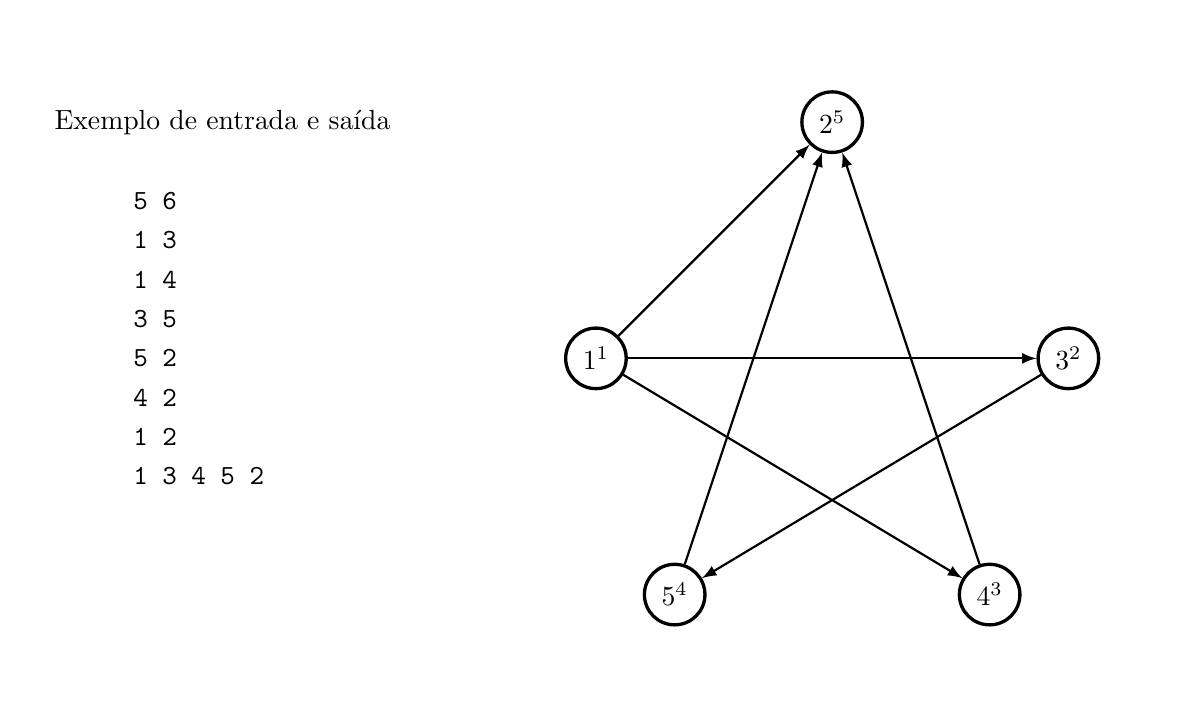
\begin{tikzpicture}
\node[draw,opacity=0] at (0, 0) {x};
\node[draw,opacity=0] at (14, 8) {x};

	\node[anchor=west] (header) at (0, 7.0) { \bbbold{Exemplo de entrada e saída} };


	\node[anchor=west] (line1) at (1.0, 6.0) { \bbtext{\texttt{5 6} } };







	\node[draw,very thick,circle] (node1) at (7.0, 4.0) { \bbtext{1$^1$} };

	\node[draw,very thick,circle] (node2) at (10.0, 7.0) { \bbtext{2$^5$} };

	\node[draw,very thick,circle] (node3) at (13.0, 4.0) { \bbtext{3$^2$} };

	\node[draw,very thick,circle] (node4) at (12.0, 1.0) { \bbtext{4$^3$} };

	\node[draw,very thick,circle] (node5) at (8.0, 1.0) { \bbtext{5$^4$} };

	\node[anchor=west] (line2) at (1.0, 5.5) { \bbtext{\texttt{1 3} } };






	\draw[thick,-latex](node1) to (node3);


	\node[anchor=west] (line3) at (1.0, 5.0) { \bbtext{\texttt{1 4} } };


	\draw[thick,-latex](node1) to (node4);


	\node[anchor=west] (line4) at (1.0, 4.5) { \bbtext{\texttt{3 5} } };


	\draw[thick,-latex](node3) to (node5);

	\node[anchor=west] (line5) at (1.0, 4.0) { \bbtext{\texttt{5 2} } };


	\draw[thick,-latex](node5) to (node2);


	\node[anchor=west] (line6) at (1.0, 3.5) { \bbtext{\texttt{4 2} } };


	\draw[thick,-latex](node4) to (node2);


	\node[anchor=west] (line7) at (1.0, 3.0) { \bbtext{\texttt{1 2} } };


	\draw[thick,-latex](node1) to (node2);


	\node[anchor=west] (line8) at (1.0, 2.5) { \bbtext{\texttt{1 3 4 5 2} } };





\end{tikzpicture}
\end{frame}
\begin{frame}[plain,t]
\begin{tikzpicture}
\node[draw,opacity=0] at (0, 0) {x};
\node[draw,opacity=0] at (14, 8) {x};

	\node[anchor=west] (header) at (0, 7.0) { \bbbold{Exemplo de entrada e saída} };


	\node[anchor=west] (line1) at (1.0, 6.0) { \bbtext{\texttt{5 6} } };







	\node[draw,very thick,circle] (node1) at (7.0, 4.0) { \bbtext{1$^1$} };

	\node[draw,very thick,circle] (node2) at (10.0, 7.0) { \bbtext{2$^5$} };

	\node[draw,very thick,circle] (node3) at (13.0, 4.0) { \bbtext{3$^2$} };

	\node[draw,very thick,circle] (node4) at (12.0, 1.0) { \bbtext{4$^3$} };

	\node[draw,very thick,circle] (node5) at (8.0, 1.0) { \bbtext{5$^4$} };

	\node[anchor=west] (line2) at (1.0, 5.5) { \bbtext{\texttt{1 3} } };






	\draw[thick,-latex,color=BBOrange](node1) to (node3);


	\node[anchor=west] (line3) at (1.0, 5.0) { \bbtext{\texttt{1 4} } };


	\draw[thick,-latex](node1) to (node4);


	\node[anchor=west] (line4) at (1.0, 4.5) { \bbtext{\texttt{3 5} } };


	\draw[thick,-latex](node3) to (node5);

	\node[anchor=west] (line5) at (1.0, 4.0) { \bbtext{\texttt{5 2} } };


	\draw[thick,-latex](node5) to (node2);


	\node[anchor=west] (line6) at (1.0, 3.5) { \bbtext{\texttt{4 2} } };


	\draw[thick,-latex](node4) to (node2);


	\node[anchor=west] (line7) at (1.0, 3.0) { \bbtext{\texttt{1 2} } };


	\draw[thick,-latex](node1) to (node2);


	\node[anchor=west] (line8) at (1.0, 2.5) { \bbtext{\texttt{1 3 4 5 2} } };






\end{tikzpicture}
\end{frame}
\begin{frame}[plain,t]
\begin{tikzpicture}
\node[draw,opacity=0] at (0, 0) {x};
\node[draw,opacity=0] at (14, 8) {x};

	\node[anchor=west] (header) at (0, 7.0) { \bbbold{Exemplo de entrada e saída} };


	\node[anchor=west] (line1) at (1.0, 6.0) { \bbtext{\texttt{5 6} } };







	\node[draw,very thick,circle] (node1) at (7.0, 4.0) { \bbtext{1$^1$} };

	\node[draw,very thick,circle] (node2) at (10.0, 7.0) { \bbtext{2$^5$} };

	\node[draw,very thick,circle] (node3) at (13.0, 4.0) { \bbtext{3$^2$} };

	\node[draw,very thick,circle] (node4) at (12.0, 1.0) { \bbtext{4$^3$} };

	\node[draw,very thick,circle] (node5) at (8.0, 1.0) { \bbtext{5$^4$} };

	\node[anchor=west] (line2) at (1.0, 5.5) { \bbtext{\texttt{1 3}\ \ \textcolor{BBGreen}{\faCheck} } };






	\draw[thick,-latex,color=BBOrange](node1) to (node3);


	\node[anchor=west] (line3) at (1.0, 5.0) { \bbtext{\texttt{1 4} } };


	\draw[thick,-latex](node1) to (node4);


	\node[anchor=west] (line4) at (1.0, 4.5) { \bbtext{\texttt{3 5} } };


	\draw[thick,-latex](node3) to (node5);

	\node[anchor=west] (line5) at (1.0, 4.0) { \bbtext{\texttt{5 2} } };


	\draw[thick,-latex](node5) to (node2);


	\node[anchor=west] (line6) at (1.0, 3.5) { \bbtext{\texttt{4 2} } };


	\draw[thick,-latex](node4) to (node2);


	\node[anchor=west] (line7) at (1.0, 3.0) { \bbtext{\texttt{1 2} } };


	\draw[thick,-latex](node1) to (node2);


	\node[anchor=west] (line8) at (1.0, 2.5) { \bbtext{\texttt{1 3 4 5 2} } };







\end{tikzpicture}
\end{frame}
\begin{frame}[plain,t]
\begin{tikzpicture}
\node[draw,opacity=0] at (0, 0) {x};
\node[draw,opacity=0] at (14, 8) {x};

	\node[anchor=west] (header) at (0, 7.0) { \bbbold{Exemplo de entrada e saída} };


	\node[anchor=west] (line1) at (1.0, 6.0) { \bbtext{\texttt{5 6} } };







	\node[draw,very thick,circle] (node1) at (7.0, 4.0) { \bbtext{1$^1$} };

	\node[draw,very thick,circle] (node2) at (10.0, 7.0) { \bbtext{2$^5$} };

	\node[draw,very thick,circle] (node3) at (13.0, 4.0) { \bbtext{3$^2$} };

	\node[draw,very thick,circle] (node4) at (12.0, 1.0) { \bbtext{4$^3$} };

	\node[draw,very thick,circle] (node5) at (8.0, 1.0) { \bbtext{5$^4$} };

	\node[anchor=west] (line2) at (1.0, 5.5) { \bbtext{\texttt{1 3}\ \ \textcolor{BBGreen}{\faCheck} } };






	\draw[thick,-latex,color=BBBlack](node1) to (node3);


	\node[anchor=west] (line3) at (1.0, 5.0) { \bbtext{\texttt{1 4} } };


	\draw[thick,-latex,color=BBOrange](node1) to (node4);


	\node[anchor=west] (line4) at (1.0, 4.5) { \bbtext{\texttt{3 5} } };


	\draw[thick,-latex](node3) to (node5);

	\node[anchor=west] (line5) at (1.0, 4.0) { \bbtext{\texttt{5 2} } };


	\draw[thick,-latex](node5) to (node2);


	\node[anchor=west] (line6) at (1.0, 3.5) { \bbtext{\texttt{4 2} } };


	\draw[thick,-latex](node4) to (node2);


	\node[anchor=west] (line7) at (1.0, 3.0) { \bbtext{\texttt{1 2} } };


	\draw[thick,-latex](node1) to (node2);


	\node[anchor=west] (line8) at (1.0, 2.5) { \bbtext{\texttt{1 3 4 5 2} } };








\end{tikzpicture}
\end{frame}
\begin{frame}[plain,t]
\begin{tikzpicture}
\node[draw,opacity=0] at (0, 0) {x};
\node[draw,opacity=0] at (14, 8) {x};

	\node[anchor=west] (header) at (0, 7.0) { \bbbold{Exemplo de entrada e saída} };


	\node[anchor=west] (line1) at (1.0, 6.0) { \bbtext{\texttt{5 6} } };







	\node[draw,very thick,circle] (node1) at (7.0, 4.0) { \bbtext{1$^1$} };

	\node[draw,very thick,circle] (node2) at (10.0, 7.0) { \bbtext{2$^5$} };

	\node[draw,very thick,circle] (node3) at (13.0, 4.0) { \bbtext{3$^2$} };

	\node[draw,very thick,circle] (node4) at (12.0, 1.0) { \bbtext{4$^3$} };

	\node[draw,very thick,circle] (node5) at (8.0, 1.0) { \bbtext{5$^4$} };

	\node[anchor=west] (line2) at (1.0, 5.5) { \bbtext{\texttt{1 3}\ \ \textcolor{BBGreen}{\faCheck} } };






	\draw[thick,-latex,color=BBBlack](node1) to (node3);


	\node[anchor=west] (line3) at (1.0, 5.0) { \bbtext{\texttt{1 4}\ \ \textcolor{BBGreen}{\faCheck} } };


	\draw[thick,-latex,color=BBOrange](node1) to (node4);


	\node[anchor=west] (line4) at (1.0, 4.5) { \bbtext{\texttt{3 5} } };


	\draw[thick,-latex](node3) to (node5);

	\node[anchor=west] (line5) at (1.0, 4.0) { \bbtext{\texttt{5 2} } };


	\draw[thick,-latex](node5) to (node2);


	\node[anchor=west] (line6) at (1.0, 3.5) { \bbtext{\texttt{4 2} } };


	\draw[thick,-latex](node4) to (node2);


	\node[anchor=west] (line7) at (1.0, 3.0) { \bbtext{\texttt{1 2} } };


	\draw[thick,-latex](node1) to (node2);


	\node[anchor=west] (line8) at (1.0, 2.5) { \bbtext{\texttt{1 3 4 5 2} } };









\end{tikzpicture}
\end{frame}
\begin{frame}[plain,t]
\begin{tikzpicture}
\node[draw,opacity=0] at (0, 0) {x};
\node[draw,opacity=0] at (14, 8) {x};

	\node[anchor=west] (header) at (0, 7.0) { \bbbold{Exemplo de entrada e saída} };


	\node[anchor=west] (line1) at (1.0, 6.0) { \bbtext{\texttt{5 6} } };







	\node[draw,very thick,circle] (node1) at (7.0, 4.0) { \bbtext{1$^1$} };

	\node[draw,very thick,circle] (node2) at (10.0, 7.0) { \bbtext{2$^5$} };

	\node[draw,very thick,circle] (node3) at (13.0, 4.0) { \bbtext{3$^2$} };

	\node[draw,very thick,circle] (node4) at (12.0, 1.0) { \bbtext{4$^3$} };

	\node[draw,very thick,circle] (node5) at (8.0, 1.0) { \bbtext{5$^4$} };

	\node[anchor=west] (line2) at (1.0, 5.5) { \bbtext{\texttt{1 3}\ \ \textcolor{BBGreen}{\faCheck} } };






	\draw[thick,-latex,color=BBBlack](node1) to (node3);


	\node[anchor=west] (line3) at (1.0, 5.0) { \bbtext{\texttt{1 4}\ \ \textcolor{BBGreen}{\faCheck} } };


	\draw[thick,-latex,color=BBBlack](node1) to (node4);


	\node[anchor=west] (line4) at (1.0, 4.5) { \bbtext{\texttt{3 5} } };


	\draw[thick,-latex,color=BBOrange](node3) to (node5);

	\node[anchor=west] (line5) at (1.0, 4.0) { \bbtext{\texttt{5 2} } };


	\draw[thick,-latex](node5) to (node2);


	\node[anchor=west] (line6) at (1.0, 3.5) { \bbtext{\texttt{4 2} } };


	\draw[thick,-latex](node4) to (node2);


	\node[anchor=west] (line7) at (1.0, 3.0) { \bbtext{\texttt{1 2} } };


	\draw[thick,-latex](node1) to (node2);


	\node[anchor=west] (line8) at (1.0, 2.5) { \bbtext{\texttt{1 3 4 5 2} } };










\end{tikzpicture}
\end{frame}
\begin{frame}[plain,t]
\begin{tikzpicture}
\node[draw,opacity=0] at (0, 0) {x};
\node[draw,opacity=0] at (14, 8) {x};

	\node[anchor=west] (header) at (0, 7.0) { \bbbold{Exemplo de entrada e saída} };


	\node[anchor=west] (line1) at (1.0, 6.0) { \bbtext{\texttt{5 6} } };







	\node[draw,very thick,circle] (node1) at (7.0, 4.0) { \bbtext{1$^1$} };

	\node[draw,very thick,circle] (node2) at (10.0, 7.0) { \bbtext{2$^5$} };

	\node[draw,very thick,circle] (node3) at (13.0, 4.0) { \bbtext{3$^2$} };

	\node[draw,very thick,circle] (node4) at (12.0, 1.0) { \bbtext{4$^3$} };

	\node[draw,very thick,circle] (node5) at (8.0, 1.0) { \bbtext{5$^4$} };

	\node[anchor=west] (line2) at (1.0, 5.5) { \bbtext{\texttt{1 3}\ \ \textcolor{BBGreen}{\faCheck} } };






	\draw[thick,-latex,color=BBBlack](node1) to (node3);


	\node[anchor=west] (line3) at (1.0, 5.0) { \bbtext{\texttt{1 4}\ \ \textcolor{BBGreen}{\faCheck} } };


	\draw[thick,-latex,color=BBBlack](node1) to (node4);


	\node[anchor=west] (line4) at (1.0, 4.5) { \bbtext{\texttt{3 5}\ \ \textcolor{BBGreen}{\faCheck} } };


	\draw[thick,-latex,color=BBOrange](node3) to (node5);

	\node[anchor=west] (line5) at (1.0, 4.0) { \bbtext{\texttt{5 2} } };


	\draw[thick,-latex](node5) to (node2);


	\node[anchor=west] (line6) at (1.0, 3.5) { \bbtext{\texttt{4 2} } };


	\draw[thick,-latex](node4) to (node2);


	\node[anchor=west] (line7) at (1.0, 3.0) { \bbtext{\texttt{1 2} } };


	\draw[thick,-latex](node1) to (node2);


	\node[anchor=west] (line8) at (1.0, 2.5) { \bbtext{\texttt{1 3 4 5 2} } };











\end{tikzpicture}
\end{frame}
\begin{frame}[plain,t]
\begin{tikzpicture}
\node[draw,opacity=0] at (0, 0) {x};
\node[draw,opacity=0] at (14, 8) {x};

	\node[anchor=west] (header) at (0, 7.0) { \bbbold{Exemplo de entrada e saída} };


	\node[anchor=west] (line1) at (1.0, 6.0) { \bbtext{\texttt{5 6} } };







	\node[draw,very thick,circle] (node1) at (7.0, 4.0) { \bbtext{1$^1$} };

	\node[draw,very thick,circle] (node2) at (10.0, 7.0) { \bbtext{2$^5$} };

	\node[draw,very thick,circle] (node3) at (13.0, 4.0) { \bbtext{3$^2$} };

	\node[draw,very thick,circle] (node4) at (12.0, 1.0) { \bbtext{4$^3$} };

	\node[draw,very thick,circle] (node5) at (8.0, 1.0) { \bbtext{5$^4$} };

	\node[anchor=west] (line2) at (1.0, 5.5) { \bbtext{\texttt{1 3}\ \ \textcolor{BBGreen}{\faCheck} } };






	\draw[thick,-latex,color=BBBlack](node1) to (node3);


	\node[anchor=west] (line3) at (1.0, 5.0) { \bbtext{\texttt{1 4}\ \ \textcolor{BBGreen}{\faCheck} } };


	\draw[thick,-latex,color=BBBlack](node1) to (node4);


	\node[anchor=west] (line4) at (1.0, 4.5) { \bbtext{\texttt{3 5}\ \ \textcolor{BBGreen}{\faCheck} } };


	\draw[thick,-latex,color=BBBlack](node3) to (node5);

	\node[anchor=west] (line5) at (1.0, 4.0) { \bbtext{\texttt{5 2} } };


	\draw[thick,-latex,color=BBOrange](node5) to (node2);


	\node[anchor=west] (line6) at (1.0, 3.5) { \bbtext{\texttt{4 2} } };


	\draw[thick,-latex](node4) to (node2);


	\node[anchor=west] (line7) at (1.0, 3.0) { \bbtext{\texttt{1 2} } };


	\draw[thick,-latex](node1) to (node2);


	\node[anchor=west] (line8) at (1.0, 2.5) { \bbtext{\texttt{1 3 4 5 2} } };












\end{tikzpicture}
\end{frame}
\begin{frame}[plain,t]
\begin{tikzpicture}
\node[draw,opacity=0] at (0, 0) {x};
\node[draw,opacity=0] at (14, 8) {x};

	\node[anchor=west] (header) at (0, 7.0) { \bbbold{Exemplo de entrada e saída} };


	\node[anchor=west] (line1) at (1.0, 6.0) { \bbtext{\texttt{5 6} } };







	\node[draw,very thick,circle] (node1) at (7.0, 4.0) { \bbtext{1$^1$} };

	\node[draw,very thick,circle] (node2) at (10.0, 7.0) { \bbtext{2$^5$} };

	\node[draw,very thick,circle] (node3) at (13.0, 4.0) { \bbtext{3$^2$} };

	\node[draw,very thick,circle] (node4) at (12.0, 1.0) { \bbtext{4$^3$} };

	\node[draw,very thick,circle] (node5) at (8.0, 1.0) { \bbtext{5$^4$} };

	\node[anchor=west] (line2) at (1.0, 5.5) { \bbtext{\texttt{1 3}\ \ \textcolor{BBGreen}{\faCheck} } };






	\draw[thick,-latex,color=BBBlack](node1) to (node3);


	\node[anchor=west] (line3) at (1.0, 5.0) { \bbtext{\texttt{1 4}\ \ \textcolor{BBGreen}{\faCheck} } };


	\draw[thick,-latex,color=BBBlack](node1) to (node4);


	\node[anchor=west] (line4) at (1.0, 4.5) { \bbtext{\texttt{3 5}\ \ \textcolor{BBGreen}{\faCheck} } };


	\draw[thick,-latex,color=BBBlack](node3) to (node5);

	\node[anchor=west] (line5) at (1.0, 4.0) { \bbtext{\texttt{5 2}\ \ \textcolor{BBGreen}{\faCheck} } };


	\draw[thick,-latex,color=BBOrange](node5) to (node2);


	\node[anchor=west] (line6) at (1.0, 3.5) { \bbtext{\texttt{4 2} } };


	\draw[thick,-latex](node4) to (node2);


	\node[anchor=west] (line7) at (1.0, 3.0) { \bbtext{\texttt{1 2} } };


	\draw[thick,-latex](node1) to (node2);


	\node[anchor=west] (line8) at (1.0, 2.5) { \bbtext{\texttt{1 3 4 5 2} } };













\end{tikzpicture}
\end{frame}
\begin{frame}[plain,t]
\begin{tikzpicture}
\node[draw,opacity=0] at (0, 0) {x};
\node[draw,opacity=0] at (14, 8) {x};

	\node[anchor=west] (header) at (0, 7.0) { \bbbold{Exemplo de entrada e saída} };


	\node[anchor=west] (line1) at (1.0, 6.0) { \bbtext{\texttt{5 6} } };







	\node[draw,very thick,circle] (node1) at (7.0, 4.0) { \bbtext{1$^1$} };

	\node[draw,very thick,circle] (node2) at (10.0, 7.0) { \bbtext{2$^5$} };

	\node[draw,very thick,circle] (node3) at (13.0, 4.0) { \bbtext{3$^2$} };

	\node[draw,very thick,circle] (node4) at (12.0, 1.0) { \bbtext{4$^3$} };

	\node[draw,very thick,circle] (node5) at (8.0, 1.0) { \bbtext{5$^4$} };

	\node[anchor=west] (line2) at (1.0, 5.5) { \bbtext{\texttt{1 3}\ \ \textcolor{BBGreen}{\faCheck} } };






	\draw[thick,-latex,color=BBBlack](node1) to (node3);


	\node[anchor=west] (line3) at (1.0, 5.0) { \bbtext{\texttt{1 4}\ \ \textcolor{BBGreen}{\faCheck} } };


	\draw[thick,-latex,color=BBBlack](node1) to (node4);


	\node[anchor=west] (line4) at (1.0, 4.5) { \bbtext{\texttt{3 5}\ \ \textcolor{BBGreen}{\faCheck} } };


	\draw[thick,-latex,color=BBBlack](node3) to (node5);

	\node[anchor=west] (line5) at (1.0, 4.0) { \bbtext{\texttt{5 2}\ \ \textcolor{BBGreen}{\faCheck} } };


	\draw[thick,-latex,color=BBBlack](node5) to (node2);


	\node[anchor=west] (line6) at (1.0, 3.5) { \bbtext{\texttt{4 2} } };


	\draw[thick,-latex,color=BBOrange](node4) to (node2);


	\node[anchor=west] (line7) at (1.0, 3.0) { \bbtext{\texttt{1 2} } };


	\draw[thick,-latex](node1) to (node2);


	\node[anchor=west] (line8) at (1.0, 2.5) { \bbtext{\texttt{1 3 4 5 2} } };














\end{tikzpicture}
\end{frame}
\begin{frame}[plain,t]
\begin{tikzpicture}
\node[draw,opacity=0] at (0, 0) {x};
\node[draw,opacity=0] at (14, 8) {x};

	\node[anchor=west] (header) at (0, 7.0) { \bbbold{Exemplo de entrada e saída} };


	\node[anchor=west] (line1) at (1.0, 6.0) { \bbtext{\texttt{5 6} } };







	\node[draw,very thick,circle] (node1) at (7.0, 4.0) { \bbtext{1$^1$} };

	\node[draw,very thick,circle] (node2) at (10.0, 7.0) { \bbtext{2$^5$} };

	\node[draw,very thick,circle] (node3) at (13.0, 4.0) { \bbtext{3$^2$} };

	\node[draw,very thick,circle] (node4) at (12.0, 1.0) { \bbtext{4$^3$} };

	\node[draw,very thick,circle] (node5) at (8.0, 1.0) { \bbtext{5$^4$} };

	\node[anchor=west] (line2) at (1.0, 5.5) { \bbtext{\texttt{1 3}\ \ \textcolor{BBGreen}{\faCheck} } };






	\draw[thick,-latex,color=BBBlack](node1) to (node3);


	\node[anchor=west] (line3) at (1.0, 5.0) { \bbtext{\texttt{1 4}\ \ \textcolor{BBGreen}{\faCheck} } };


	\draw[thick,-latex,color=BBBlack](node1) to (node4);


	\node[anchor=west] (line4) at (1.0, 4.5) { \bbtext{\texttt{3 5}\ \ \textcolor{BBGreen}{\faCheck} } };


	\draw[thick,-latex,color=BBBlack](node3) to (node5);

	\node[anchor=west] (line5) at (1.0, 4.0) { \bbtext{\texttt{5 2}\ \ \textcolor{BBGreen}{\faCheck} } };


	\draw[thick,-latex,color=BBBlack](node5) to (node2);


	\node[anchor=west] (line6) at (1.0, 3.5) { \bbtext{\texttt{4 2}\ \ \textcolor{BBGreen}{\faCheck} } };


	\draw[thick,-latex,color=BBOrange](node4) to (node2);


	\node[anchor=west] (line7) at (1.0, 3.0) { \bbtext{\texttt{1 2} } };


	\draw[thick,-latex](node1) to (node2);


	\node[anchor=west] (line8) at (1.0, 2.5) { \bbtext{\texttt{1 3 4 5 2} } };















\end{tikzpicture}
\end{frame}
\begin{frame}[plain,t]
\begin{tikzpicture}
\node[draw,opacity=0] at (0, 0) {x};
\node[draw,opacity=0] at (14, 8) {x};

	\node[anchor=west] (header) at (0, 7.0) { \bbbold{Exemplo de entrada e saída} };


	\node[anchor=west] (line1) at (1.0, 6.0) { \bbtext{\texttt{5 6} } };







	\node[draw,very thick,circle] (node1) at (7.0, 4.0) { \bbtext{1$^1$} };

	\node[draw,very thick,circle] (node2) at (10.0, 7.0) { \bbtext{2$^5$} };

	\node[draw,very thick,circle] (node3) at (13.0, 4.0) { \bbtext{3$^2$} };

	\node[draw,very thick,circle] (node4) at (12.0, 1.0) { \bbtext{4$^3$} };

	\node[draw,very thick,circle] (node5) at (8.0, 1.0) { \bbtext{5$^4$} };

	\node[anchor=west] (line2) at (1.0, 5.5) { \bbtext{\texttt{1 3}\ \ \textcolor{BBGreen}{\faCheck} } };






	\draw[thick,-latex,color=BBBlack](node1) to (node3);


	\node[anchor=west] (line3) at (1.0, 5.0) { \bbtext{\texttt{1 4}\ \ \textcolor{BBGreen}{\faCheck} } };


	\draw[thick,-latex,color=BBBlack](node1) to (node4);


	\node[anchor=west] (line4) at (1.0, 4.5) { \bbtext{\texttt{3 5}\ \ \textcolor{BBGreen}{\faCheck} } };


	\draw[thick,-latex,color=BBBlack](node3) to (node5);

	\node[anchor=west] (line5) at (1.0, 4.0) { \bbtext{\texttt{5 2}\ \ \textcolor{BBGreen}{\faCheck} } };


	\draw[thick,-latex,color=BBBlack](node5) to (node2);


	\node[anchor=west] (line6) at (1.0, 3.5) { \bbtext{\texttt{4 2}\ \ \textcolor{BBGreen}{\faCheck} } };


	\draw[thick,-latex,color=BBBlack](node4) to (node2);


	\node[anchor=west] (line7) at (1.0, 3.0) { \bbtext{\texttt{1 2} } };


	\draw[thick,-latex,color=BBOrange](node1) to (node2);


	\node[anchor=west] (line8) at (1.0, 2.5) { \bbtext{\texttt{1 3 4 5 2} } };
















\end{tikzpicture}
\end{frame}
\begin{frame}[plain,t]
\begin{tikzpicture}
\node[draw,opacity=0] at (0, 0) {x};
\node[draw,opacity=0] at (14, 8) {x};

	\node[anchor=west] (header) at (0, 7.0) { \bbbold{Exemplo de entrada e saída} };


	\node[anchor=west] (line1) at (1.0, 6.0) { \bbtext{\texttt{5 6} } };







	\node[draw,very thick,circle] (node1) at (7.0, 4.0) { \bbtext{1$^1$} };

	\node[draw,very thick,circle] (node2) at (10.0, 7.0) { \bbtext{2$^5$} };

	\node[draw,very thick,circle] (node3) at (13.0, 4.0) { \bbtext{3$^2$} };

	\node[draw,very thick,circle] (node4) at (12.0, 1.0) { \bbtext{4$^3$} };

	\node[draw,very thick,circle] (node5) at (8.0, 1.0) { \bbtext{5$^4$} };

	\node[anchor=west] (line2) at (1.0, 5.5) { \bbtext{\texttt{1 3}\ \ \textcolor{BBGreen}{\faCheck} } };






	\draw[thick,-latex,color=BBBlack](node1) to (node3);


	\node[anchor=west] (line3) at (1.0, 5.0) { \bbtext{\texttt{1 4}\ \ \textcolor{BBGreen}{\faCheck} } };


	\draw[thick,-latex,color=BBBlack](node1) to (node4);


	\node[anchor=west] (line4) at (1.0, 4.5) { \bbtext{\texttt{3 5}\ \ \textcolor{BBGreen}{\faCheck} } };


	\draw[thick,-latex,color=BBBlack](node3) to (node5);

	\node[anchor=west] (line5) at (1.0, 4.0) { \bbtext{\texttt{5 2}\ \ \textcolor{BBGreen}{\faCheck} } };


	\draw[thick,-latex,color=BBBlack](node5) to (node2);


	\node[anchor=west] (line6) at (1.0, 3.5) { \bbtext{\texttt{4 2}\ \ \textcolor{BBGreen}{\faCheck} } };


	\draw[thick,-latex,color=BBBlack](node4) to (node2);


	\node[anchor=west] (line7) at (1.0, 3.0) { \bbtext{\texttt{1 2}\ \ \textcolor{BBGreen}{\faCheck} } };


	\draw[thick,-latex,color=BBOrange](node1) to (node2);


	\node[anchor=west] (line8) at (1.0, 2.5) { \bbtext{\texttt{1 3 4 5 2} } };

















\end{tikzpicture}
\end{frame}
\begin{frame}[plain,t]
\begin{tikzpicture}
\node[draw,opacity=0] at (0, 0) {x};
\node[draw,opacity=0] at (14, 8) {x};

	\node[anchor=west] (header) at (0, 7.0) { \bbbold{Exemplo de entrada e saída} };


	\node[anchor=west] (line1) at (1.0, 6.0) { \bbtext{\texttt{5 6} } };


	\draw[->,color=BBBlack,-latex,very thick] (2.05, 2.25) to  (2.05, 1.25);

	\node[] (r) at (2.05, 1.0) { \footnotesize \bboutput{YES} };




	\node[draw,very thick,circle] (node1) at (7.0, 4.0) { \bbtext{1$^1$} };

	\node[draw,very thick,circle] (node2) at (10.0, 7.0) { \bbtext{2$^5$} };

	\node[draw,very thick,circle] (node3) at (13.0, 4.0) { \bbtext{3$^2$} };

	\node[draw,very thick,circle] (node4) at (12.0, 1.0) { \bbtext{4$^3$} };

	\node[draw,very thick,circle] (node5) at (8.0, 1.0) { \bbtext{5$^4$} };

	\node[anchor=west] (line2) at (1.0, 5.5) { \bbtext{\texttt{1 3}\ \ \textcolor{BBGreen}{\faCheck} } };






	\draw[thick,-latex,color=BBBlack](node1) to (node3);


	\node[anchor=west] (line3) at (1.0, 5.0) { \bbtext{\texttt{1 4}\ \ \textcolor{BBGreen}{\faCheck} } };


	\draw[thick,-latex,color=BBBlack](node1) to (node4);


	\node[anchor=west] (line4) at (1.0, 4.5) { \bbtext{\texttt{3 5}\ \ \textcolor{BBGreen}{\faCheck} } };


	\draw[thick,-latex,color=BBBlack](node3) to (node5);

	\node[anchor=west] (line5) at (1.0, 4.0) { \bbtext{\texttt{5 2}\ \ \textcolor{BBGreen}{\faCheck} } };


	\draw[thick,-latex,color=BBBlack](node5) to (node2);


	\node[anchor=west] (line6) at (1.0, 3.5) { \bbtext{\texttt{4 2}\ \ \textcolor{BBGreen}{\faCheck} } };


	\draw[thick,-latex,color=BBBlack](node4) to (node2);


	\node[anchor=west] (line7) at (1.0, 3.0) { \bbtext{\texttt{1 2}\ \ \textcolor{BBGreen}{\faCheck} } };


	\draw[thick,-latex,color=BBOrange](node1) to (node2);


	\node[anchor=west] (line8) at (1.0, 2.5) { \bbtext{\texttt{1 3 4 5 2} } };



















\end{tikzpicture}
\end{frame}
\begin{frame}[plain,t]
\begin{tikzpicture}
\node[draw,opacity=0] at (0, 0) {x};
\node[draw,opacity=0] at (14, 8) {x};

	\node[anchor=west] (header) at (0, 7.0) { \bbbold{Exemplo de entrada e saída} };

\end{tikzpicture}
\end{frame}
\begin{frame}[plain,t]
\begin{tikzpicture}
\node[draw,opacity=0] at (0, 0) {x};
\node[draw,opacity=0] at (14, 8) {x};

	\node[anchor=west] (header) at (0, 7.0) { \bbbold{Exemplo de entrada e saída} };


	\node[anchor=west] (line1) at (1.0, 6.0) { \bbtext{\texttt{5 6} } };

\end{tikzpicture}
\end{frame}
\begin{frame}[plain,t]
\begin{tikzpicture}
\node[draw,opacity=0] at (0, 0) {x};
\node[draw,opacity=0] at (14, 8) {x};

	\node[anchor=west] (header) at (0, 7.0) { \bbbold{Exemplo de entrada e saída} };


	\node[anchor=west] (line1) at (1.0, 6.0) { \bbtext{\texttt{5 6} } };





	\node[draw,very thick,circle] (node1) at (7.0, 4.0) { \bbtext{1} };

	\node[draw,very thick,circle] (node2) at (10.0, 7.0) { \bbtext{2} };

	\node[draw,very thick,circle] (node3) at (13.0, 4.0) { \bbtext{3} };

	\node[draw,very thick,circle] (node4) at (12.0, 1.0) { \bbtext{4} };

	\node[draw,very thick,circle] (node5) at (8.0, 1.0) { \bbtext{5} };
\end{tikzpicture}
\end{frame}
\begin{frame}[plain,t]
\begin{tikzpicture}
\node[draw,opacity=0] at (0, 0) {x};
\node[draw,opacity=0] at (14, 8) {x};

	\node[anchor=west] (header) at (0, 7.0) { \bbbold{Exemplo de entrada e saída} };


	\node[anchor=west] (line1) at (1.0, 6.0) { \bbtext{\texttt{5 6} } };





	\node[draw,very thick,circle] (node1) at (7.0, 4.0) { \bbtext{1} };

	\node[draw,very thick,circle] (node2) at (10.0, 7.0) { \bbtext{2} };

	\node[draw,very thick,circle] (node3) at (13.0, 4.0) { \bbtext{3} };

	\node[draw,very thick,circle] (node4) at (12.0, 1.0) { \bbtext{4} };

	\node[draw,very thick,circle] (node5) at (8.0, 1.0) { \bbtext{5} };

	\node[anchor=west] (line2) at (1.0, 5.5) { \bbtext{\texttt{1 3} } };

\end{tikzpicture}
\end{frame}
\begin{frame}[plain,t]
\begin{tikzpicture}
\node[draw,opacity=0] at (0, 0) {x};
\node[draw,opacity=0] at (14, 8) {x};

	\node[anchor=west] (header) at (0, 7.0) { \bbbold{Exemplo de entrada e saída} };


	\node[anchor=west] (line1) at (1.0, 6.0) { \bbtext{\texttt{5 6} } };





	\node[draw,very thick,circle] (node1) at (7.0, 4.0) { \bbtext{1} };

	\node[draw,very thick,circle] (node2) at (10.0, 7.0) { \bbtext{2} };

	\node[draw,very thick,circle] (node3) at (13.0, 4.0) { \bbtext{3} };

	\node[draw,very thick,circle] (node4) at (12.0, 1.0) { \bbtext{4} };

	\node[draw,very thick,circle] (node5) at (8.0, 1.0) { \bbtext{5} };

	\node[anchor=west] (line2) at (1.0, 5.5) { \bbtext{\texttt{1 3} } };





	\draw[thick,-latex](node1) to (node3);

\end{tikzpicture}
\end{frame}
\begin{frame}[plain,t]
\begin{tikzpicture}
\node[draw,opacity=0] at (0, 0) {x};
\node[draw,opacity=0] at (14, 8) {x};

	\node[anchor=west] (header) at (0, 7.0) { \bbbold{Exemplo de entrada e saída} };


	\node[anchor=west] (line1) at (1.0, 6.0) { \bbtext{\texttt{5 6} } };





	\node[draw,very thick,circle] (node1) at (7.0, 4.0) { \bbtext{1} };

	\node[draw,very thick,circle] (node2) at (10.0, 7.0) { \bbtext{2} };

	\node[draw,very thick,circle] (node3) at (13.0, 4.0) { \bbtext{3} };

	\node[draw,very thick,circle] (node4) at (12.0, 1.0) { \bbtext{4} };

	\node[draw,very thick,circle] (node5) at (8.0, 1.0) { \bbtext{5} };

	\node[anchor=west] (line2) at (1.0, 5.5) { \bbtext{\texttt{1 3} } };





	\draw[thick,-latex](node1) to (node3);


	\node[anchor=west] (line3) at (1.0, 5.0) { \bbtext{\texttt{1 4} } };

\end{tikzpicture}
\end{frame}
\begin{frame}[plain,t]
\begin{tikzpicture}
\node[draw,opacity=0] at (0, 0) {x};
\node[draw,opacity=0] at (14, 8) {x};

	\node[anchor=west] (header) at (0, 7.0) { \bbbold{Exemplo de entrada e saída} };


	\node[anchor=west] (line1) at (1.0, 6.0) { \bbtext{\texttt{5 6} } };





	\node[draw,very thick,circle] (node1) at (7.0, 4.0) { \bbtext{1} };

	\node[draw,very thick,circle] (node2) at (10.0, 7.0) { \bbtext{2} };

	\node[draw,very thick,circle] (node3) at (13.0, 4.0) { \bbtext{3} };

	\node[draw,very thick,circle] (node4) at (12.0, 1.0) { \bbtext{4} };

	\node[draw,very thick,circle] (node5) at (8.0, 1.0) { \bbtext{5} };

	\node[anchor=west] (line2) at (1.0, 5.5) { \bbtext{\texttt{1 3} } };





	\draw[thick,-latex](node1) to (node3);


	\node[anchor=west] (line3) at (1.0, 5.0) { \bbtext{\texttt{1 4} } };


	\draw[thick,-latex](node1) to (node4);

\end{tikzpicture}
\end{frame}
\begin{frame}[plain,t]
\begin{tikzpicture}
\node[draw,opacity=0] at (0, 0) {x};
\node[draw,opacity=0] at (14, 8) {x};

	\node[anchor=west] (header) at (0, 7.0) { \bbbold{Exemplo de entrada e saída} };


	\node[anchor=west] (line1) at (1.0, 6.0) { \bbtext{\texttt{5 6} } };





	\node[draw,very thick,circle] (node1) at (7.0, 4.0) { \bbtext{1} };

	\node[draw,very thick,circle] (node2) at (10.0, 7.0) { \bbtext{2} };

	\node[draw,very thick,circle] (node3) at (13.0, 4.0) { \bbtext{3} };

	\node[draw,very thick,circle] (node4) at (12.0, 1.0) { \bbtext{4} };

	\node[draw,very thick,circle] (node5) at (8.0, 1.0) { \bbtext{5} };

	\node[anchor=west] (line2) at (1.0, 5.5) { \bbtext{\texttt{1 3} } };





	\draw[thick,-latex](node1) to (node3);


	\node[anchor=west] (line3) at (1.0, 5.0) { \bbtext{\texttt{1 4} } };


	\draw[thick,-latex](node1) to (node4);


	\node[anchor=west] (line4) at (1.0, 4.5) { \bbtext{\texttt{3 5} } };

\end{tikzpicture}
\end{frame}
\begin{frame}[plain,t]
\begin{tikzpicture}
\node[draw,opacity=0] at (0, 0) {x};
\node[draw,opacity=0] at (14, 8) {x};

	\node[anchor=west] (header) at (0, 7.0) { \bbbold{Exemplo de entrada e saída} };


	\node[anchor=west] (line1) at (1.0, 6.0) { \bbtext{\texttt{5 6} } };





	\node[draw,very thick,circle] (node1) at (7.0, 4.0) { \bbtext{1} };

	\node[draw,very thick,circle] (node2) at (10.0, 7.0) { \bbtext{2} };

	\node[draw,very thick,circle] (node3) at (13.0, 4.0) { \bbtext{3} };

	\node[draw,very thick,circle] (node4) at (12.0, 1.0) { \bbtext{4} };

	\node[draw,very thick,circle] (node5) at (8.0, 1.0) { \bbtext{5} };

	\node[anchor=west] (line2) at (1.0, 5.5) { \bbtext{\texttt{1 3} } };





	\draw[thick,-latex](node1) to (node3);


	\node[anchor=west] (line3) at (1.0, 5.0) { \bbtext{\texttt{1 4} } };


	\draw[thick,-latex](node1) to (node4);


	\node[anchor=west] (line4) at (1.0, 4.5) { \bbtext{\texttt{3 5} } };


	\draw[thick,-latex](node3) to (node5);
\end{tikzpicture}
\end{frame}
\begin{frame}[plain,t]
\begin{tikzpicture}
\node[draw,opacity=0] at (0, 0) {x};
\node[draw,opacity=0] at (14, 8) {x};

	\node[anchor=west] (header) at (0, 7.0) { \bbbold{Exemplo de entrada e saída} };


	\node[anchor=west] (line1) at (1.0, 6.0) { \bbtext{\texttt{5 6} } };





	\node[draw,very thick,circle] (node1) at (7.0, 4.0) { \bbtext{1} };

	\node[draw,very thick,circle] (node2) at (10.0, 7.0) { \bbtext{2} };

	\node[draw,very thick,circle] (node3) at (13.0, 4.0) { \bbtext{3} };

	\node[draw,very thick,circle] (node4) at (12.0, 1.0) { \bbtext{4} };

	\node[draw,very thick,circle] (node5) at (8.0, 1.0) { \bbtext{5} };

	\node[anchor=west] (line2) at (1.0, 5.5) { \bbtext{\texttt{1 3} } };





	\draw[thick,-latex](node1) to (node3);


	\node[anchor=west] (line3) at (1.0, 5.0) { \bbtext{\texttt{1 4} } };


	\draw[thick,-latex](node1) to (node4);


	\node[anchor=west] (line4) at (1.0, 4.5) { \bbtext{\texttt{3 5} } };


	\draw[thick,-latex](node3) to (node5);

	\node[anchor=west] (line5) at (1.0, 4.0) { \bbtext{\texttt{5 2} } };

\end{tikzpicture}
\end{frame}
\begin{frame}[plain,t]
\begin{tikzpicture}
\node[draw,opacity=0] at (0, 0) {x};
\node[draw,opacity=0] at (14, 8) {x};

	\node[anchor=west] (header) at (0, 7.0) { \bbbold{Exemplo de entrada e saída} };


	\node[anchor=west] (line1) at (1.0, 6.0) { \bbtext{\texttt{5 6} } };





	\node[draw,very thick,circle] (node1) at (7.0, 4.0) { \bbtext{1} };

	\node[draw,very thick,circle] (node2) at (10.0, 7.0) { \bbtext{2} };

	\node[draw,very thick,circle] (node3) at (13.0, 4.0) { \bbtext{3} };

	\node[draw,very thick,circle] (node4) at (12.0, 1.0) { \bbtext{4} };

	\node[draw,very thick,circle] (node5) at (8.0, 1.0) { \bbtext{5} };

	\node[anchor=west] (line2) at (1.0, 5.5) { \bbtext{\texttt{1 3} } };





	\draw[thick,-latex](node1) to (node3);


	\node[anchor=west] (line3) at (1.0, 5.0) { \bbtext{\texttt{1 4} } };


	\draw[thick,-latex](node1) to (node4);


	\node[anchor=west] (line4) at (1.0, 4.5) { \bbtext{\texttt{3 5} } };


	\draw[thick,-latex](node3) to (node5);

	\node[anchor=west] (line5) at (1.0, 4.0) { \bbtext{\texttt{5 2} } };


	\draw[thick,-latex](node5) to (node2);

\end{tikzpicture}
\end{frame}
\begin{frame}[plain,t]
\begin{tikzpicture}
\node[draw,opacity=0] at (0, 0) {x};
\node[draw,opacity=0] at (14, 8) {x};

	\node[anchor=west] (header) at (0, 7.0) { \bbbold{Exemplo de entrada e saída} };


	\node[anchor=west] (line1) at (1.0, 6.0) { \bbtext{\texttt{5 6} } };





	\node[draw,very thick,circle] (node1) at (7.0, 4.0) { \bbtext{1} };

	\node[draw,very thick,circle] (node2) at (10.0, 7.0) { \bbtext{2} };

	\node[draw,very thick,circle] (node3) at (13.0, 4.0) { \bbtext{3} };

	\node[draw,very thick,circle] (node4) at (12.0, 1.0) { \bbtext{4} };

	\node[draw,very thick,circle] (node5) at (8.0, 1.0) { \bbtext{5} };

	\node[anchor=west] (line2) at (1.0, 5.5) { \bbtext{\texttt{1 3} } };





	\draw[thick,-latex](node1) to (node3);


	\node[anchor=west] (line3) at (1.0, 5.0) { \bbtext{\texttt{1 4} } };


	\draw[thick,-latex](node1) to (node4);


	\node[anchor=west] (line4) at (1.0, 4.5) { \bbtext{\texttt{3 5} } };


	\draw[thick,-latex](node3) to (node5);

	\node[anchor=west] (line5) at (1.0, 4.0) { \bbtext{\texttt{5 2} } };


	\draw[thick,-latex](node5) to (node2);


	\node[anchor=west] (line6) at (1.0, 3.5) { \bbtext{\texttt{4 2} } };

\end{tikzpicture}
\end{frame}
\begin{frame}[plain,t]
\begin{tikzpicture}
\node[draw,opacity=0] at (0, 0) {x};
\node[draw,opacity=0] at (14, 8) {x};

	\node[anchor=west] (header) at (0, 7.0) { \bbbold{Exemplo de entrada e saída} };


	\node[anchor=west] (line1) at (1.0, 6.0) { \bbtext{\texttt{5 6} } };





	\node[draw,very thick,circle] (node1) at (7.0, 4.0) { \bbtext{1} };

	\node[draw,very thick,circle] (node2) at (10.0, 7.0) { \bbtext{2} };

	\node[draw,very thick,circle] (node3) at (13.0, 4.0) { \bbtext{3} };

	\node[draw,very thick,circle] (node4) at (12.0, 1.0) { \bbtext{4} };

	\node[draw,very thick,circle] (node5) at (8.0, 1.0) { \bbtext{5} };

	\node[anchor=west] (line2) at (1.0, 5.5) { \bbtext{\texttt{1 3} } };





	\draw[thick,-latex](node1) to (node3);


	\node[anchor=west] (line3) at (1.0, 5.0) { \bbtext{\texttt{1 4} } };


	\draw[thick,-latex](node1) to (node4);


	\node[anchor=west] (line4) at (1.0, 4.5) { \bbtext{\texttt{3 5} } };


	\draw[thick,-latex](node3) to (node5);

	\node[anchor=west] (line5) at (1.0, 4.0) { \bbtext{\texttt{5 2} } };


	\draw[thick,-latex](node5) to (node2);


	\node[anchor=west] (line6) at (1.0, 3.5) { \bbtext{\texttt{4 2} } };


	\draw[thick,-latex](node4) to (node2);

\end{tikzpicture}
\end{frame}
\begin{frame}[plain,t]
\begin{tikzpicture}
\node[draw,opacity=0] at (0, 0) {x};
\node[draw,opacity=0] at (14, 8) {x};

	\node[anchor=west] (header) at (0, 7.0) { \bbbold{Exemplo de entrada e saída} };


	\node[anchor=west] (line1) at (1.0, 6.0) { \bbtext{\texttt{5 6} } };





	\node[draw,very thick,circle] (node1) at (7.0, 4.0) { \bbtext{1} };

	\node[draw,very thick,circle] (node2) at (10.0, 7.0) { \bbtext{2} };

	\node[draw,very thick,circle] (node3) at (13.0, 4.0) { \bbtext{3} };

	\node[draw,very thick,circle] (node4) at (12.0, 1.0) { \bbtext{4} };

	\node[draw,very thick,circle] (node5) at (8.0, 1.0) { \bbtext{5} };

	\node[anchor=west] (line2) at (1.0, 5.5) { \bbtext{\texttt{1 3} } };





	\draw[thick,-latex](node1) to (node3);


	\node[anchor=west] (line3) at (1.0, 5.0) { \bbtext{\texttt{1 4} } };


	\draw[thick,-latex](node1) to (node4);


	\node[anchor=west] (line4) at (1.0, 4.5) { \bbtext{\texttt{3 5} } };


	\draw[thick,-latex](node3) to (node5);

	\node[anchor=west] (line5) at (1.0, 4.0) { \bbtext{\texttt{5 2} } };


	\draw[thick,-latex](node5) to (node2);


	\node[anchor=west] (line6) at (1.0, 3.5) { \bbtext{\texttt{4 2} } };


	\draw[thick,-latex](node4) to (node2);


	\node[anchor=west] (line7) at (1.0, 3.0) { \bbtext{\texttt{1 2} } };

\end{tikzpicture}
\end{frame}
\begin{frame}[plain,t]
\begin{tikzpicture}
\node[draw,opacity=0] at (0, 0) {x};
\node[draw,opacity=0] at (14, 8) {x};

	\node[anchor=west] (header) at (0, 7.0) { \bbbold{Exemplo de entrada e saída} };


	\node[anchor=west] (line1) at (1.0, 6.0) { \bbtext{\texttt{5 6} } };





	\node[draw,very thick,circle] (node1) at (7.0, 4.0) { \bbtext{1} };

	\node[draw,very thick,circle] (node2) at (10.0, 7.0) { \bbtext{2} };

	\node[draw,very thick,circle] (node3) at (13.0, 4.0) { \bbtext{3} };

	\node[draw,very thick,circle] (node4) at (12.0, 1.0) { \bbtext{4} };

	\node[draw,very thick,circle] (node5) at (8.0, 1.0) { \bbtext{5} };

	\node[anchor=west] (line2) at (1.0, 5.5) { \bbtext{\texttt{1 3} } };





	\draw[thick,-latex](node1) to (node3);


	\node[anchor=west] (line3) at (1.0, 5.0) { \bbtext{\texttt{1 4} } };


	\draw[thick,-latex](node1) to (node4);


	\node[anchor=west] (line4) at (1.0, 4.5) { \bbtext{\texttt{3 5} } };


	\draw[thick,-latex](node3) to (node5);

	\node[anchor=west] (line5) at (1.0, 4.0) { \bbtext{\texttt{5 2} } };


	\draw[thick,-latex](node5) to (node2);


	\node[anchor=west] (line6) at (1.0, 3.5) { \bbtext{\texttt{4 2} } };


	\draw[thick,-latex](node4) to (node2);


	\node[anchor=west] (line7) at (1.0, 3.0) { \bbtext{\texttt{1 2} } };


	\draw[thick,-latex](node1) to (node2);

\end{tikzpicture}
\end{frame}
\begin{frame}[plain,t]
\begin{tikzpicture}
\node[draw,opacity=0] at (0, 0) {x};
\node[draw,opacity=0] at (14, 8) {x};

	\node[anchor=west] (header) at (0, 7.0) { \bbbold{Exemplo de entrada e saída} };


	\node[anchor=west] (line1) at (1.0, 6.0) { \bbtext{\texttt{5 6} } };





	\node[draw,very thick,circle] (node1) at (7.0, 4.0) { \bbtext{1} };

	\node[draw,very thick,circle] (node2) at (10.0, 7.0) { \bbtext{2} };

	\node[draw,very thick,circle] (node3) at (13.0, 4.0) { \bbtext{3} };

	\node[draw,very thick,circle] (node4) at (12.0, 1.0) { \bbtext{4} };

	\node[draw,very thick,circle] (node5) at (8.0, 1.0) { \bbtext{5} };

	\node[anchor=west] (line2) at (1.0, 5.5) { \bbtext{\texttt{1 3} } };





	\draw[thick,-latex](node1) to (node3);


	\node[anchor=west] (line3) at (1.0, 5.0) { \bbtext{\texttt{1 4} } };


	\draw[thick,-latex](node1) to (node4);


	\node[anchor=west] (line4) at (1.0, 4.5) { \bbtext{\texttt{3 5} } };


	\draw[thick,-latex](node3) to (node5);

	\node[anchor=west] (line5) at (1.0, 4.0) { \bbtext{\texttt{5 2} } };


	\draw[thick,-latex](node5) to (node2);


	\node[anchor=west] (line6) at (1.0, 3.5) { \bbtext{\texttt{4 2} } };


	\draw[thick,-latex](node4) to (node2);


	\node[anchor=west] (line7) at (1.0, 3.0) { \bbtext{\texttt{1 2} } };


	\draw[thick,-latex](node1) to (node2);


	\node[anchor=west] (line8) at (1.0, 2.5) { \bbtext{\texttt{1 2 4 5 3} } };

\end{tikzpicture}
\end{frame}
\begin{frame}[plain,t]
\begin{tikzpicture}
\node[draw,opacity=0] at (0, 0) {x};
\node[draw,opacity=0] at (14, 8) {x};

	\node[anchor=west] (header) at (0, 7.0) { \bbbold{Exemplo de entrada e saída} };


	\node[anchor=west] (line1) at (1.0, 6.0) { \bbtext{\texttt{5 6} } };





	\node[draw,very thick,circle] (node1) at (7.0, 4.0) { \bbtext{1$^1$} };

	\node[draw,very thick,circle] (node2) at (10.0, 7.0) { \bbtext{2$^2$} };

	\node[draw,very thick,circle] (node3) at (13.0, 4.0) { \bbtext{3$^5$} };

	\node[draw,very thick,circle] (node4) at (12.0, 1.0) { \bbtext{4$^3$} };

	\node[draw,very thick,circle] (node5) at (8.0, 1.0) { \bbtext{5$^4$} };

	\node[anchor=west] (line2) at (1.0, 5.5) { \bbtext{\texttt{1 3} } };





	\draw[thick,-latex](node1) to (node3);


	\node[anchor=west] (line3) at (1.0, 5.0) { \bbtext{\texttt{1 4} } };


	\draw[thick,-latex](node1) to (node4);


	\node[anchor=west] (line4) at (1.0, 4.5) { \bbtext{\texttt{3 5} } };


	\draw[thick,-latex](node3) to (node5);

	\node[anchor=west] (line5) at (1.0, 4.0) { \bbtext{\texttt{5 2} } };


	\draw[thick,-latex](node5) to (node2);


	\node[anchor=west] (line6) at (1.0, 3.5) { \bbtext{\texttt{4 2} } };


	\draw[thick,-latex](node4) to (node2);


	\node[anchor=west] (line7) at (1.0, 3.0) { \bbtext{\texttt{1 2} } };


	\draw[thick,-latex](node1) to (node2);


	\node[anchor=west] (line8) at (1.0, 2.5) { \bbtext{\texttt{1 2 4 5 3} } };




\end{tikzpicture}
\end{frame}
\begin{frame}[plain,t]
\begin{tikzpicture}
\node[draw,opacity=0] at (0, 0) {x};
\node[draw,opacity=0] at (14, 8) {x};

	\node[anchor=west] (header) at (0, 7.0) { \bbbold{Exemplo de entrada e saída} };


	\node[anchor=west] (line1) at (1.0, 6.0) { \bbtext{\texttt{5 6} } };





	\node[draw,very thick,circle] (node1) at (7.0, 4.0) { \bbtext{1$^1$} };

	\node[draw,very thick,circle] (node2) at (10.0, 7.0) { \bbtext{2$^2$} };

	\node[draw,very thick,circle] (node3) at (13.0, 4.0) { \bbtext{3$^5$} };

	\node[draw,very thick,circle] (node4) at (12.0, 1.0) { \bbtext{4$^3$} };

	\node[draw,very thick,circle] (node5) at (8.0, 1.0) { \bbtext{5$^4$} };

	\node[anchor=west] (line2) at (1.0, 5.5) { \bbtext{\texttt{1 3} } };





	\draw[thick,-latex,color=BBOrange](node1) to (node3);


	\node[anchor=west] (line3) at (1.0, 5.0) { \bbtext{\texttt{1 4} } };


	\draw[thick,-latex](node1) to (node4);


	\node[anchor=west] (line4) at (1.0, 4.5) { \bbtext{\texttt{3 5} } };


	\draw[thick,-latex](node3) to (node5);

	\node[anchor=west] (line5) at (1.0, 4.0) { \bbtext{\texttt{5 2} } };


	\draw[thick,-latex](node5) to (node2);


	\node[anchor=west] (line6) at (1.0, 3.5) { \bbtext{\texttt{4 2} } };


	\draw[thick,-latex](node4) to (node2);


	\node[anchor=west] (line7) at (1.0, 3.0) { \bbtext{\texttt{1 2} } };


	\draw[thick,-latex](node1) to (node2);


	\node[anchor=west] (line8) at (1.0, 2.5) { \bbtext{\texttt{1 2 4 5 3} } };





\end{tikzpicture}
\end{frame}
\begin{frame}[plain,t]
\begin{tikzpicture}
\node[draw,opacity=0] at (0, 0) {x};
\node[draw,opacity=0] at (14, 8) {x};

	\node[anchor=west] (header) at (0, 7.0) { \bbbold{Exemplo de entrada e saída} };


	\node[anchor=west] (line1) at (1.0, 6.0) { \bbtext{\texttt{5 6} } };





	\node[draw,very thick,circle] (node1) at (7.0, 4.0) { \bbtext{1$^1$} };

	\node[draw,very thick,circle] (node2) at (10.0, 7.0) { \bbtext{2$^2$} };

	\node[draw,very thick,circle] (node3) at (13.0, 4.0) { \bbtext{3$^5$} };

	\node[draw,very thick,circle] (node4) at (12.0, 1.0) { \bbtext{4$^3$} };

	\node[draw,very thick,circle] (node5) at (8.0, 1.0) { \bbtext{5$^4$} };

	\node[anchor=west] (line2) at (1.0, 5.5) { \bbtext{\texttt{1 3}\ \ \textcolor{BBGreen}{\faCheck} } };





	\draw[thick,-latex,color=BBOrange](node1) to (node3);


	\node[anchor=west] (line3) at (1.0, 5.0) { \bbtext{\texttt{1 4} } };


	\draw[thick,-latex](node1) to (node4);


	\node[anchor=west] (line4) at (1.0, 4.5) { \bbtext{\texttt{3 5} } };


	\draw[thick,-latex](node3) to (node5);

	\node[anchor=west] (line5) at (1.0, 4.0) { \bbtext{\texttt{5 2} } };


	\draw[thick,-latex](node5) to (node2);


	\node[anchor=west] (line6) at (1.0, 3.5) { \bbtext{\texttt{4 2} } };


	\draw[thick,-latex](node4) to (node2);


	\node[anchor=west] (line7) at (1.0, 3.0) { \bbtext{\texttt{1 2} } };


	\draw[thick,-latex](node1) to (node2);


	\node[anchor=west] (line8) at (1.0, 2.5) { \bbtext{\texttt{1 2 4 5 3} } };






\end{tikzpicture}
\end{frame}
\begin{frame}[plain,t]
\begin{tikzpicture}
\node[draw,opacity=0] at (0, 0) {x};
\node[draw,opacity=0] at (14, 8) {x};

	\node[anchor=west] (header) at (0, 7.0) { \bbbold{Exemplo de entrada e saída} };


	\node[anchor=west] (line1) at (1.0, 6.0) { \bbtext{\texttt{5 6} } };





	\node[draw,very thick,circle] (node1) at (7.0, 4.0) { \bbtext{1$^1$} };

	\node[draw,very thick,circle] (node2) at (10.0, 7.0) { \bbtext{2$^2$} };

	\node[draw,very thick,circle] (node3) at (13.0, 4.0) { \bbtext{3$^5$} };

	\node[draw,very thick,circle] (node4) at (12.0, 1.0) { \bbtext{4$^3$} };

	\node[draw,very thick,circle] (node5) at (8.0, 1.0) { \bbtext{5$^4$} };

	\node[anchor=west] (line2) at (1.0, 5.5) { \bbtext{\texttt{1 3}\ \ \textcolor{BBGreen}{\faCheck} } };





	\draw[thick,-latex,color=BBBlack](node1) to (node3);


	\node[anchor=west] (line3) at (1.0, 5.0) { \bbtext{\texttt{1 4} } };


	\draw[thick,-latex,color=BBOrange](node1) to (node4);


	\node[anchor=west] (line4) at (1.0, 4.5) { \bbtext{\texttt{3 5} } };


	\draw[thick,-latex](node3) to (node5);

	\node[anchor=west] (line5) at (1.0, 4.0) { \bbtext{\texttt{5 2} } };


	\draw[thick,-latex](node5) to (node2);


	\node[anchor=west] (line6) at (1.0, 3.5) { \bbtext{\texttt{4 2} } };


	\draw[thick,-latex](node4) to (node2);


	\node[anchor=west] (line7) at (1.0, 3.0) { \bbtext{\texttt{1 2} } };


	\draw[thick,-latex](node1) to (node2);


	\node[anchor=west] (line8) at (1.0, 2.5) { \bbtext{\texttt{1 2 4 5 3} } };







\end{tikzpicture}
\end{frame}
\begin{frame}[plain,t]
\begin{tikzpicture}
\node[draw,opacity=0] at (0, 0) {x};
\node[draw,opacity=0] at (14, 8) {x};

	\node[anchor=west] (header) at (0, 7.0) { \bbbold{Exemplo de entrada e saída} };


	\node[anchor=west] (line1) at (1.0, 6.0) { \bbtext{\texttt{5 6} } };





	\node[draw,very thick,circle] (node1) at (7.0, 4.0) { \bbtext{1$^1$} };

	\node[draw,very thick,circle] (node2) at (10.0, 7.0) { \bbtext{2$^2$} };

	\node[draw,very thick,circle] (node3) at (13.0, 4.0) { \bbtext{3$^5$} };

	\node[draw,very thick,circle] (node4) at (12.0, 1.0) { \bbtext{4$^3$} };

	\node[draw,very thick,circle] (node5) at (8.0, 1.0) { \bbtext{5$^4$} };

	\node[anchor=west] (line2) at (1.0, 5.5) { \bbtext{\texttt{1 3}\ \ \textcolor{BBGreen}{\faCheck} } };





	\draw[thick,-latex,color=BBBlack](node1) to (node3);


	\node[anchor=west] (line3) at (1.0, 5.0) { \bbtext{\texttt{1 4}\ \ \textcolor{BBGreen}{\faCheck} } };


	\draw[thick,-latex,color=BBOrange](node1) to (node4);


	\node[anchor=west] (line4) at (1.0, 4.5) { \bbtext{\texttt{3 5} } };


	\draw[thick,-latex](node3) to (node5);

	\node[anchor=west] (line5) at (1.0, 4.0) { \bbtext{\texttt{5 2} } };


	\draw[thick,-latex](node5) to (node2);


	\node[anchor=west] (line6) at (1.0, 3.5) { \bbtext{\texttt{4 2} } };


	\draw[thick,-latex](node4) to (node2);


	\node[anchor=west] (line7) at (1.0, 3.0) { \bbtext{\texttt{1 2} } };


	\draw[thick,-latex](node1) to (node2);


	\node[anchor=west] (line8) at (1.0, 2.5) { \bbtext{\texttt{1 2 4 5 3} } };








\end{tikzpicture}
\end{frame}
\begin{frame}[plain,t]
\begin{tikzpicture}
\node[draw,opacity=0] at (0, 0) {x};
\node[draw,opacity=0] at (14, 8) {x};

	\node[anchor=west] (header) at (0, 7.0) { \bbbold{Exemplo de entrada e saída} };


	\node[anchor=west] (line1) at (1.0, 6.0) { \bbtext{\texttt{5 6} } };





	\node[draw,very thick,circle] (node1) at (7.0, 4.0) { \bbtext{1$^1$} };

	\node[draw,very thick,circle] (node2) at (10.0, 7.0) { \bbtext{2$^2$} };

	\node[draw,very thick,circle] (node3) at (13.0, 4.0) { \bbtext{3$^5$} };

	\node[draw,very thick,circle] (node4) at (12.0, 1.0) { \bbtext{4$^3$} };

	\node[draw,very thick,circle] (node5) at (8.0, 1.0) { \bbtext{5$^4$} };

	\node[anchor=west] (line2) at (1.0, 5.5) { \bbtext{\texttt{1 3}\ \ \textcolor{BBGreen}{\faCheck} } };





	\draw[thick,-latex,color=BBBlack](node1) to (node3);


	\node[anchor=west] (line3) at (1.0, 5.0) { \bbtext{\texttt{1 4}\ \ \textcolor{BBGreen}{\faCheck} } };


	\draw[thick,-latex,color=BBBlack](node1) to (node4);


	\node[anchor=west] (line4) at (1.0, 4.5) { \bbtext{\texttt{3 5} } };


	\draw[thick,-latex,color=BBOrange](node3) to (node5);

	\node[anchor=west] (line5) at (1.0, 4.0) { \bbtext{\texttt{5 2} } };


	\draw[thick,-latex](node5) to (node2);


	\node[anchor=west] (line6) at (1.0, 3.5) { \bbtext{\texttt{4 2} } };


	\draw[thick,-latex](node4) to (node2);


	\node[anchor=west] (line7) at (1.0, 3.0) { \bbtext{\texttt{1 2} } };


	\draw[thick,-latex](node1) to (node2);


	\node[anchor=west] (line8) at (1.0, 2.5) { \bbtext{\texttt{1 2 4 5 3} } };









\end{tikzpicture}
\end{frame}
\begin{frame}[plain,t]
\begin{tikzpicture}
\node[draw,opacity=0] at (0, 0) {x};
\node[draw,opacity=0] at (14, 8) {x};

	\node[anchor=west] (header) at (0, 7.0) { \bbbold{Exemplo de entrada e saída} };


	\node[anchor=west] (line1) at (1.0, 6.0) { \bbtext{\texttt{5 6} } };





	\node[draw,very thick,circle] (node1) at (7.0, 4.0) { \bbtext{1$^1$} };

	\node[draw,very thick,circle] (node2) at (10.0, 7.0) { \bbtext{2$^2$} };

	\node[draw,very thick,circle] (node3) at (13.0, 4.0) { \bbtext{3$^5$} };

	\node[draw,very thick,circle] (node4) at (12.0, 1.0) { \bbtext{4$^3$} };

	\node[draw,very thick,circle] (node5) at (8.0, 1.0) { \bbtext{5$^4$} };

	\node[anchor=west] (line2) at (1.0, 5.5) { \bbtext{\texttt{1 3}\ \ \textcolor{BBGreen}{\faCheck} } };





	\draw[thick,-latex,color=BBBlack](node1) to (node3);


	\node[anchor=west] (line3) at (1.0, 5.0) { \bbtext{\texttt{1 4}\ \ \textcolor{BBGreen}{\faCheck} } };


	\draw[thick,-latex,color=BBBlack](node1) to (node4);


	\node[anchor=west] (line4) at (1.0, 4.5) { \bbtext{\texttt{3 5}\ \ \textcolor{BBRed}{\faClose} } };


	\draw[thick,-latex,color=BBOrange](node3) to (node5);

	\node[anchor=west] (line5) at (1.0, 4.0) { \bbtext{\texttt{5 2} } };


	\draw[thick,-latex](node5) to (node2);


	\node[anchor=west] (line6) at (1.0, 3.5) { \bbtext{\texttt{4 2} } };


	\draw[thick,-latex](node4) to (node2);


	\node[anchor=west] (line7) at (1.0, 3.0) { \bbtext{\texttt{1 2} } };


	\draw[thick,-latex](node1) to (node2);


	\node[anchor=west] (line8) at (1.0, 2.5) { \bbtext{\texttt{1 2 4 5 3} } };










\end{tikzpicture}
\end{frame}
\begin{frame}[plain,t]
\begin{tikzpicture}
\node[draw,opacity=0] at (0, 0) {x};
\node[draw,opacity=0] at (14, 8) {x};

	\node[anchor=west] (header) at (0, 7.0) { \bbbold{Exemplo de entrada e saída} };


	\node[anchor=west] (line1) at (1.0, 6.0) { \bbtext{\texttt{5 6} } };


	\draw[->,color=BBBlack,-latex,very thick] (2.05, 2.25) to  (2.05, 1.25);

	\node[] (r) at (2.05, 1.0) { \footnotesize \bboutput{NO} };


	\node[draw,very thick,circle] (node1) at (7.0, 4.0) { \bbtext{1$^1$} };

	\node[draw,very thick,circle] (node2) at (10.0, 7.0) { \bbtext{2$^2$} };

	\node[draw,very thick,circle] (node3) at (13.0, 4.0) { \bbtext{3$^5$} };

	\node[draw,very thick,circle] (node4) at (12.0, 1.0) { \bbtext{4$^3$} };

	\node[draw,very thick,circle] (node5) at (8.0, 1.0) { \bbtext{5$^4$} };

	\node[anchor=west] (line2) at (1.0, 5.5) { \bbtext{\texttt{1 3}\ \ \textcolor{BBGreen}{\faCheck} } };





	\draw[thick,-latex,color=BBBlack](node1) to (node3);


	\node[anchor=west] (line3) at (1.0, 5.0) { \bbtext{\texttt{1 4}\ \ \textcolor{BBGreen}{\faCheck} } };


	\draw[thick,-latex,color=BBBlack](node1) to (node4);


	\node[anchor=west] (line4) at (1.0, 4.5) { \bbtext{\texttt{3 5}\ \ \textcolor{BBRed}{\faClose} } };


	\draw[thick,-latex,color=BBOrange](node3) to (node5);

	\node[anchor=west] (line5) at (1.0, 4.0) { \bbtext{\texttt{5 2} } };


	\draw[thick,-latex](node5) to (node2);


	\node[anchor=west] (line6) at (1.0, 3.5) { \bbtext{\texttt{4 2} } };


	\draw[thick,-latex](node4) to (node2);


	\node[anchor=west] (line7) at (1.0, 3.0) { \bbtext{\texttt{1 2} } };


	\draw[thick,-latex](node1) to (node2);


	\node[anchor=west] (line8) at (1.0, 2.5) { \bbtext{\texttt{1 2 4 5 3} } };













\end{tikzpicture}
\end{frame}
\begin{frame}[plain,t]
\begin{tikzpicture}
\node[draw,opacity=0] at (0, 0) {x};
\node[draw,opacity=0] at (14, 8) {x};

	\node[anchor=west] (title) at (0.0, 7.5) { \Large \bbbold{Solução} };
\end{tikzpicture}
\end{frame}
\begin{frame}[plain,t]
\begin{tikzpicture}
\node[draw,opacity=0] at (0, 0) {x};
\node[draw,opacity=0] at (14, 8) {x};

	\node[anchor=west] (title) at (0.0, 7.5) { \Large \bbbold{Solução} };

	\node[anchor=west] (a) at (1.0, 6.5) { $\star$ \bbtext{O problema consiste em determinar se a ordenação proposta por Michael} };

	\node[anchor=west] (a1) at (0.5, 6.0) { \bbtext{é ou não topológica} };

\end{tikzpicture}
\end{frame}
\begin{frame}[plain,t]
\begin{tikzpicture}
\node[draw,opacity=0] at (0, 0) {x};
\node[draw,opacity=0] at (14, 8) {x};

	\node[anchor=west] (title) at (0.0, 7.5) { \Large \bbbold{Solução} };

	\node[anchor=west] (a) at (1.0, 6.5) { $\star$ \bbtext{O problema consiste em determinar se a ordenação proposta por Michael} };

	\node[anchor=west] (a1) at (0.5, 6.0) { \bbtext{é ou não topológica} };


	\node[anchor=west] (b) at (1.0, 5.0) { $\star$ \bbtext{Assim, não é preciso de fato gerar uma ordenação topológica: basta verificar} };

	\node[anchor=west] (b1) at (0.5, 4.5) { \bbtext{se a ordenação proposta atende às limitações dadas} };

\end{tikzpicture}
\end{frame}
\begin{frame}[plain,t]
\begin{tikzpicture}
\node[draw,opacity=0] at (0, 0) {x};
\node[draw,opacity=0] at (14, 8) {x};

	\node[anchor=west] (title) at (0.0, 7.5) { \Large \bbbold{Solução} };

	\node[anchor=west] (a) at (1.0, 6.5) { $\star$ \bbtext{O problema consiste em determinar se a ordenação proposta por Michael} };

	\node[anchor=west] (a1) at (0.5, 6.0) { \bbtext{é ou não topológica} };


	\node[anchor=west] (b) at (1.0, 5.0) { $\star$ \bbtext{Assim, não é preciso de fato gerar uma ordenação topológica: basta verificar} };

	\node[anchor=west] (b1) at (0.5, 4.5) { \bbtext{se a ordenação proposta atende às limitações dadas} };


	\node[anchor=west] (c) at (1.0, 3.5) { $\star$ \bbtext{Um dicionário permite identificar, de forma eficiente, a posição de uma} };

	\node[anchor=west] (c1) at (0.5, 3.0) { \bbtext{tarefa de acordo com a ordenação} };

\end{tikzpicture}
\end{frame}
\begin{frame}[plain,t]
\begin{tikzpicture}
\node[draw,opacity=0] at (0, 0) {x};
\node[draw,opacity=0] at (14, 8) {x};

	\node[anchor=west] (title) at (0.0, 7.5) { \Large \bbbold{Solução} };

	\node[anchor=west] (a) at (1.0, 6.5) { $\star$ \bbtext{O problema consiste em determinar se a ordenação proposta por Michael} };

	\node[anchor=west] (a1) at (0.5, 6.0) { \bbtext{é ou não topológica} };


	\node[anchor=west] (b) at (1.0, 5.0) { $\star$ \bbtext{Assim, não é preciso de fato gerar uma ordenação topológica: basta verificar} };

	\node[anchor=west] (b1) at (0.5, 4.5) { \bbtext{se a ordenação proposta atende às limitações dadas} };


	\node[anchor=west] (c) at (1.0, 3.5) { $\star$ \bbtext{Um dicionário permite identificar, de forma eficiente, a posição de uma} };

	\node[anchor=west] (c1) at (0.5, 3.0) { \bbtext{tarefa de acordo com a ordenação} };


	\node[anchor=west] (d) at (1.0, 2.0) { $\star$ \bbtext{Se alguma limitação for violada, a resposta será \bboutput{NO}} };

\end{tikzpicture}
\end{frame}
\begin{frame}[plain,t]
\begin{tikzpicture}
\node[draw,opacity=0] at (0, 0) {x};
\node[draw,opacity=0] at (14, 8) {x};

	\node[anchor=west] (title) at (0.0, 7.5) { \Large \bbbold{Solução} };

	\node[anchor=west] (a) at (1.0, 6.5) { $\star$ \bbtext{O problema consiste em determinar se a ordenação proposta por Michael} };

	\node[anchor=west] (a1) at (0.5, 6.0) { \bbtext{é ou não topológica} };


	\node[anchor=west] (b) at (1.0, 5.0) { $\star$ \bbtext{Assim, não é preciso de fato gerar uma ordenação topológica: basta verificar} };

	\node[anchor=west] (b1) at (0.5, 4.5) { \bbtext{se a ordenação proposta atende às limitações dadas} };


	\node[anchor=west] (c) at (1.0, 3.5) { $\star$ \bbtext{Um dicionário permite identificar, de forma eficiente, a posição de uma} };

	\node[anchor=west] (c1) at (0.5, 3.0) { \bbtext{tarefa de acordo com a ordenação} };


	\node[anchor=west] (d) at (1.0, 2.0) { $\star$ \bbtext{Se alguma limitação for violada, a resposta será \bboutput{NO}} };


	\node[anchor=west] (e) at (1.0, 1.0) { $\star$ \bbtext{\bbbold{Complexidade:} $O(N + M)$} };

\end{tikzpicture}
\end{frame}
\begin{frame}[plain,t]

\inputsnippet{cpp}{46}{59}{codes/1280.cpp}

\end{frame}
\end{document}
